% Appendix B

\chapter{Results} % Main appendix title

\label{AppendixB} % For referencing this appendix elsewhere, use \ref{AppendixB}


\pagebreak


\newgeometry{margin=1.5cm}
\begin{landscape}
\leavevmode
\section{Cluster profiles}
\label{cluster_profiles}
\begin{figure}[h!]
  \vspace{0.5em} %better style
  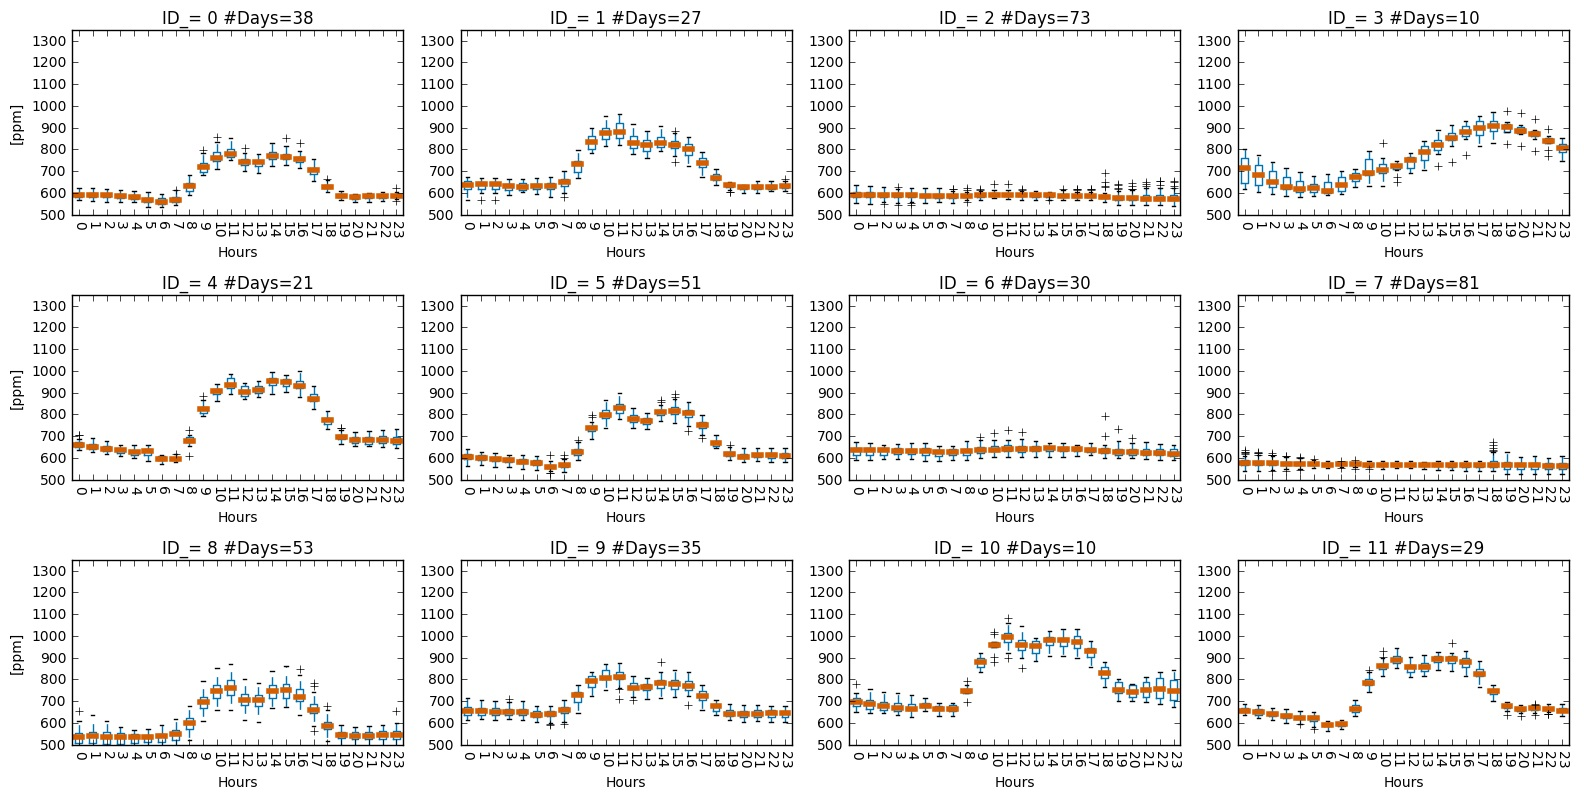
\includegraphics[scale=0.6]{Figures/candidates_CO2_NE_1.jpg}
  \caption{$CO_2$ cluster profiles for the North-East ventilation system of the building. (1/3) }
  \label{fig:candidates_profiles_NE}
\end{figure}

\begin{figure}[h!]
  \vspace{0.5em} %better style
  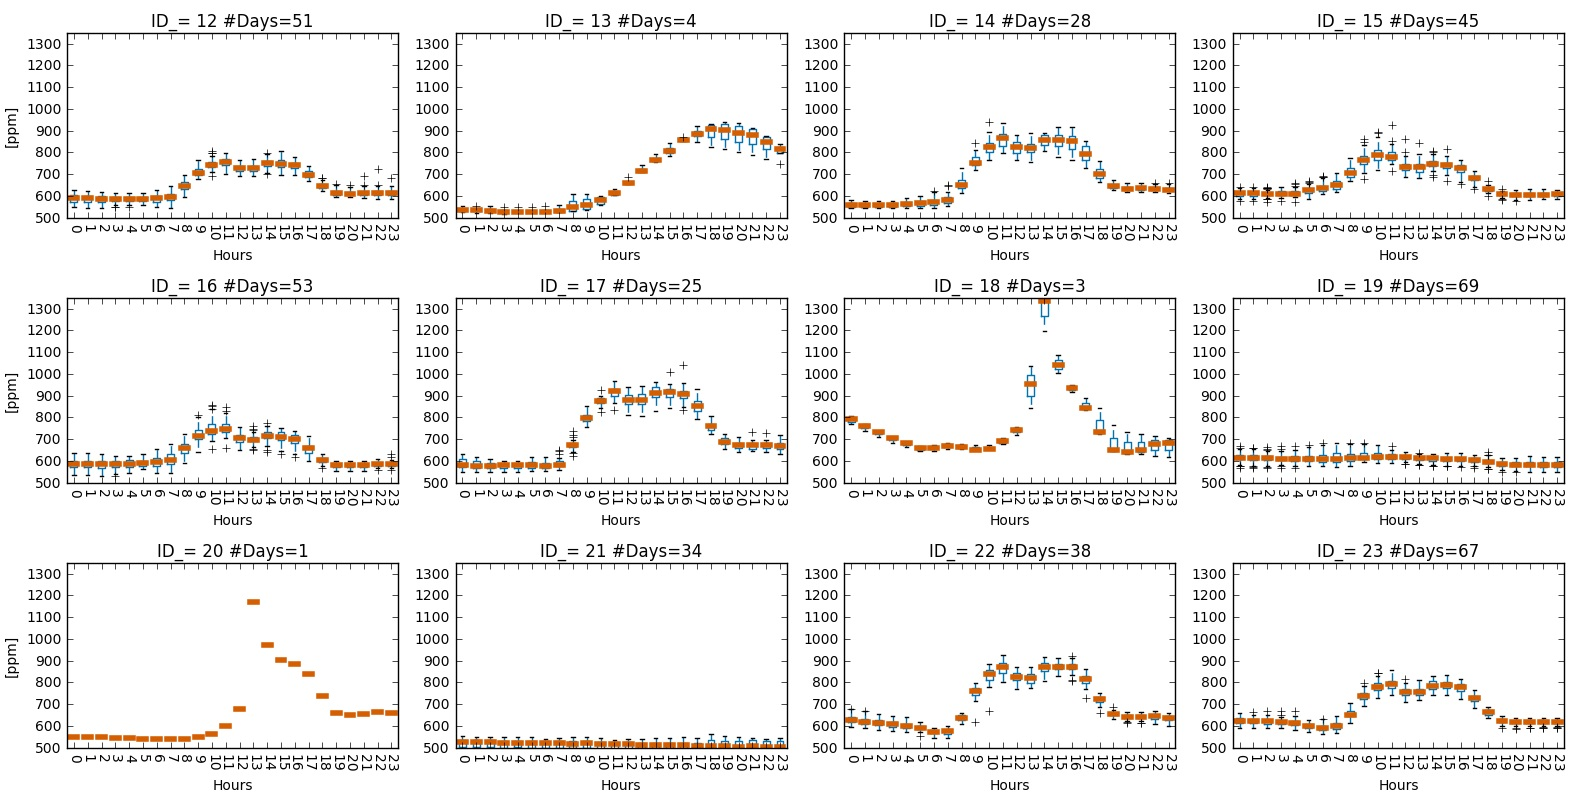
\includegraphics[scale=0.6]{Figures/candidates_CO2_NE_2.jpg}
  \caption{$CO_2$ cluster profiles for the North-East ventilation system of the building. (2/3) }
  \label{fig:candidates_profiles_NE}
\end{figure}

\begin{figure}[h!]
  \vspace{0.5em} %better style
  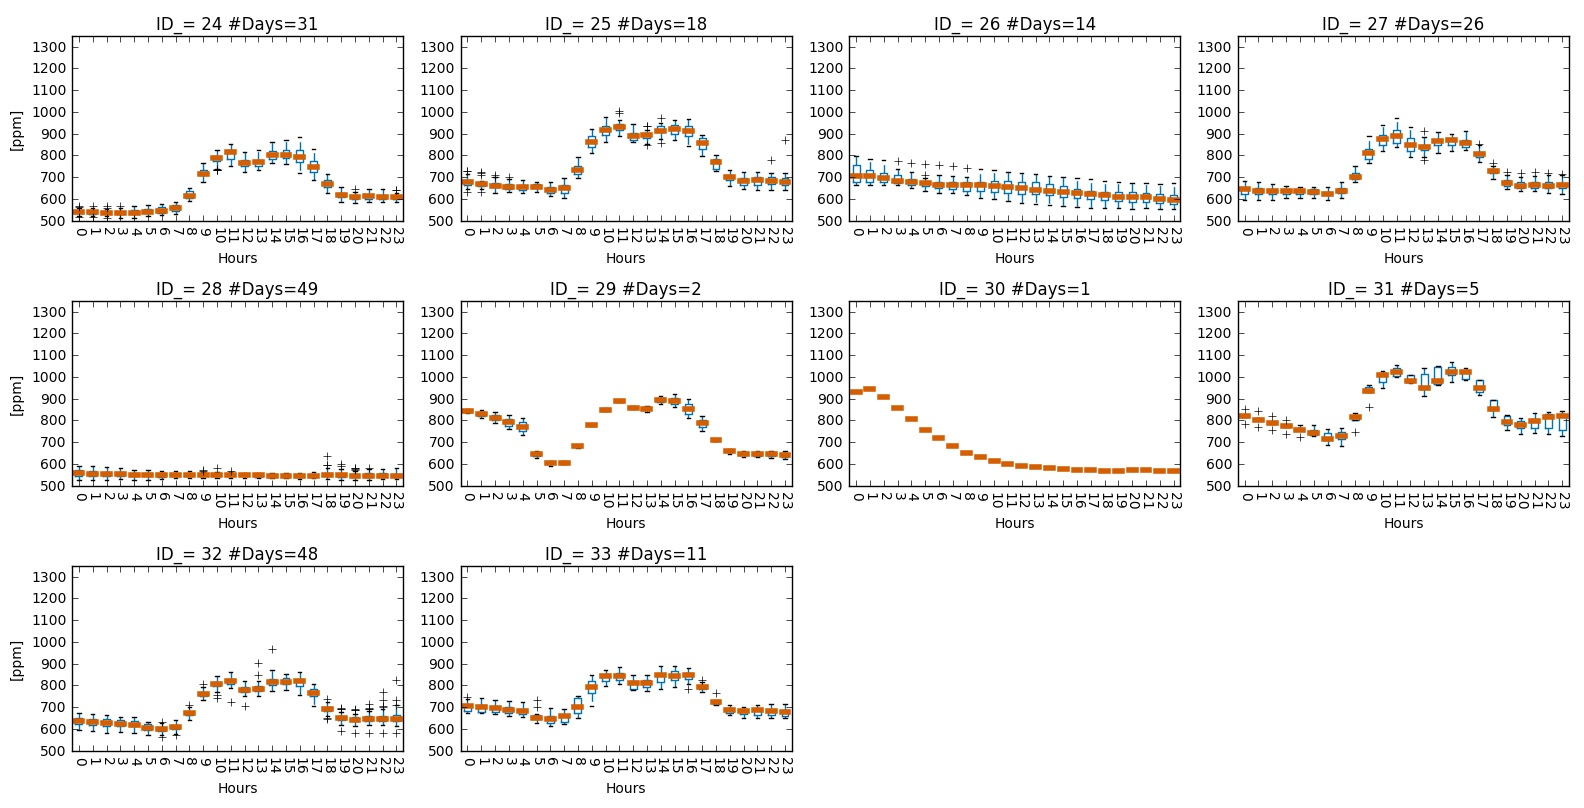
\includegraphics[scale=0.6]{Figures/candidates_CO2_NE_3.jpg}
  \caption{$CO_2$ cluster profiles for the North-East ventilation system of the building. (3/3) }
  \label{fig:candidates_profiles_NE}
\end{figure}


\begin{figure}[h!]
  \vspace{0.5em} %better style
  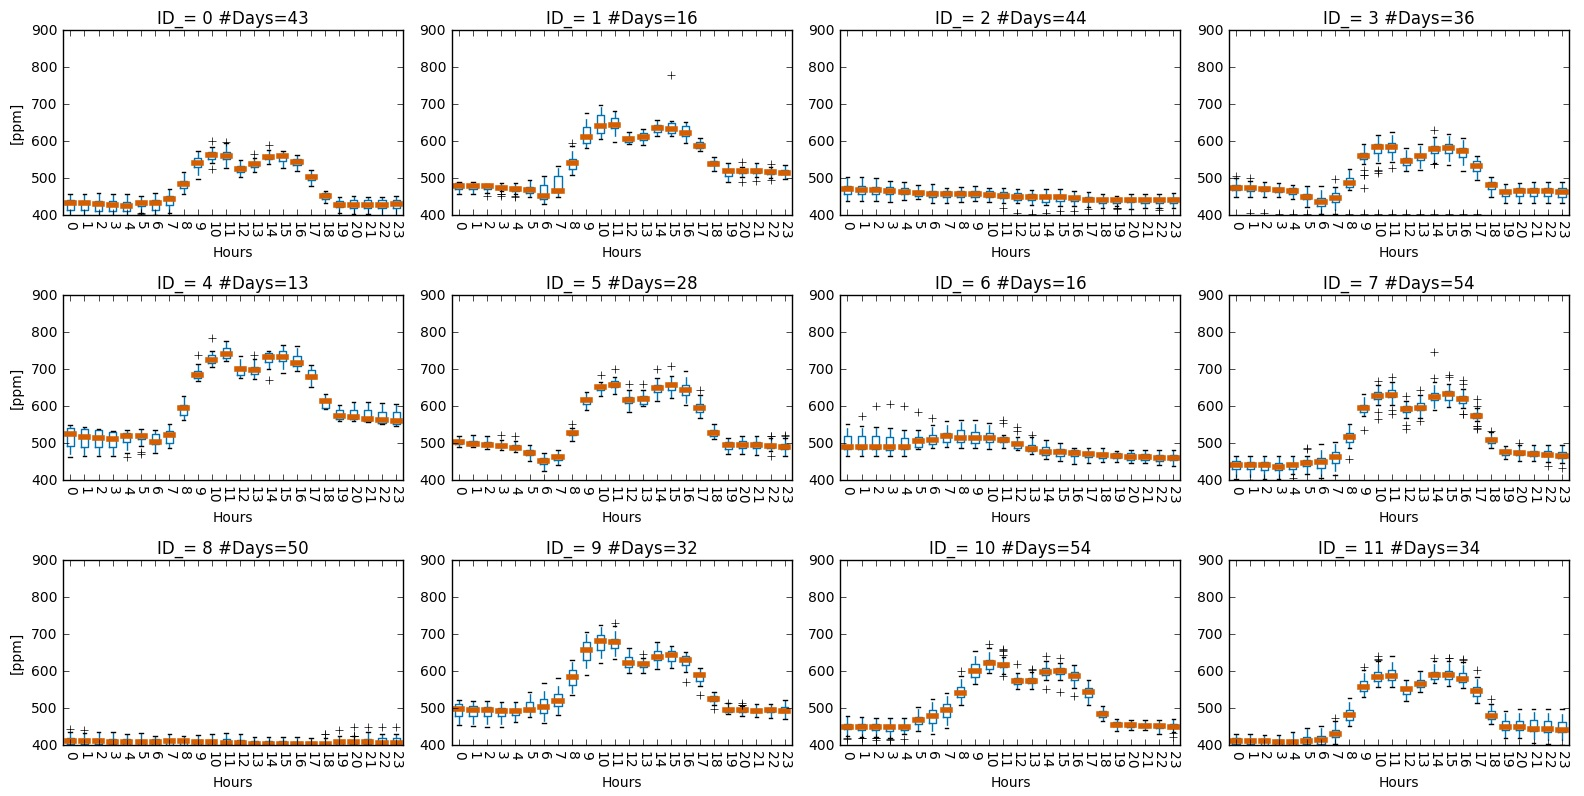
\includegraphics[scale=0.6]{Figures/candidates_CO2_SW_1.jpg}
  \caption{$CO_2$ cluster profiles for the South-West ventilation system of the building. (1/3) }
  \label{fig:candidates_profiles_SW}
\end{figure}

\begin{figure}[h!]
  \vspace{0.5em} %better style
  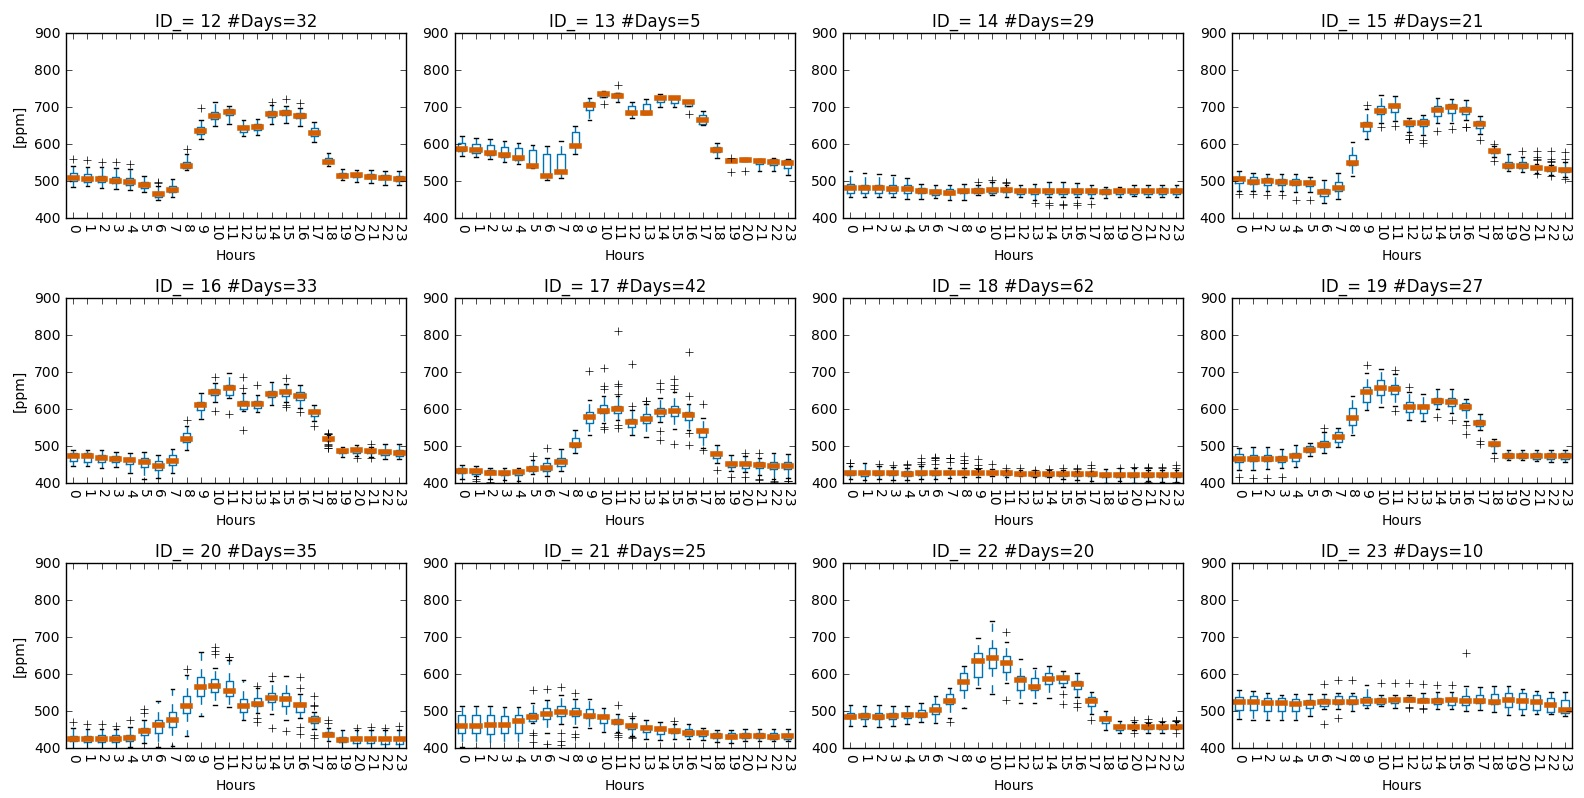
\includegraphics[scale=0.6]{Figures/candidates_CO2_SW_2.jpg}
  \caption{$CO_2$ cluster profiles for the South-West ventilation system of the building. (2/3) }
  \label{fig:candidates_profiles_SW}
\end{figure}

\begin{figure}[h!]
  \vspace{0.5em} %better style
  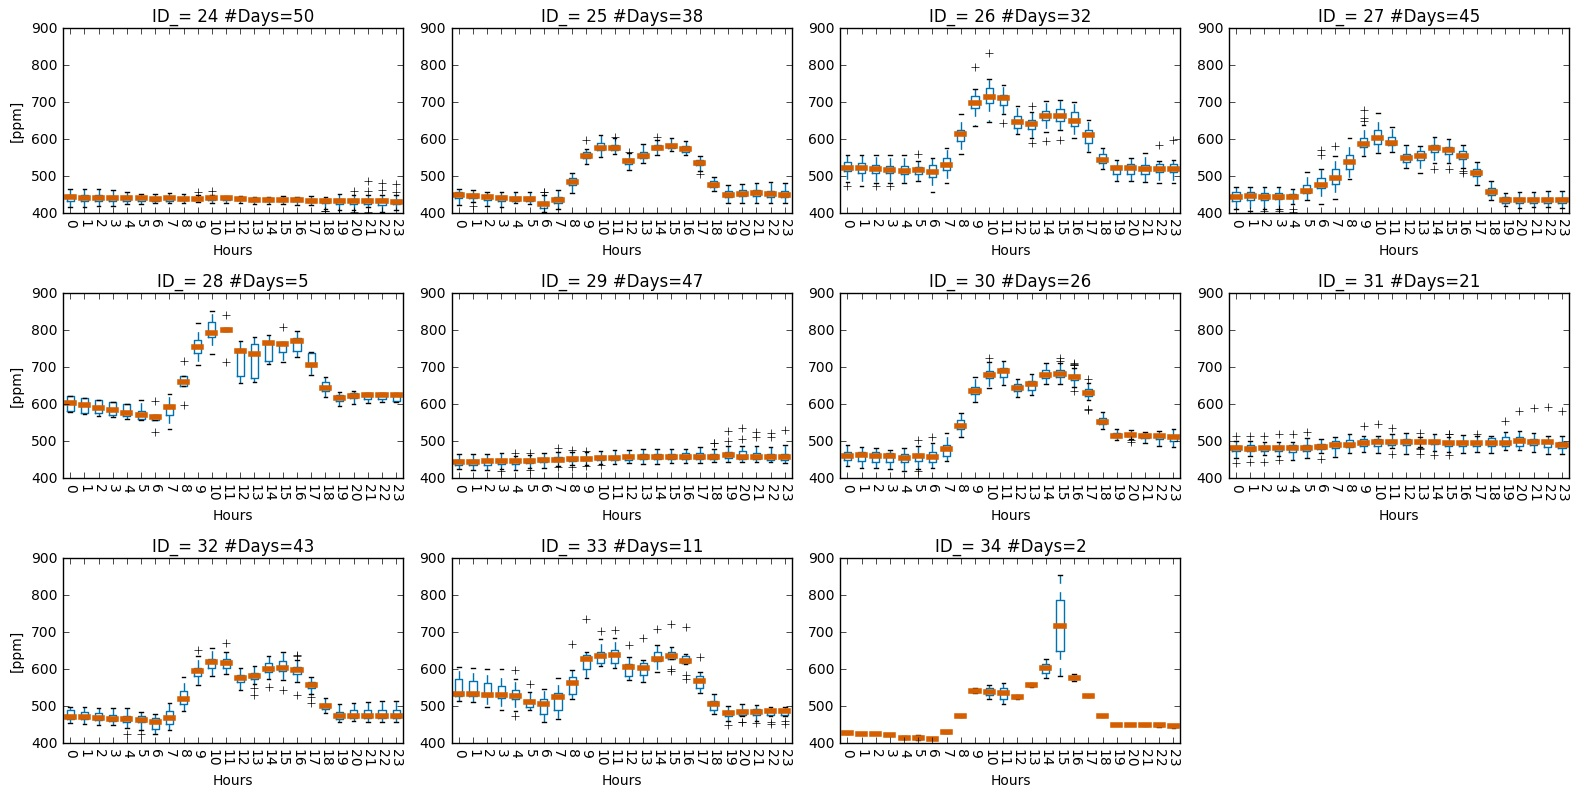
\includegraphics[scale=0.6]{Figures/candidates_CO2_SW_3.jpg}
  \caption{$CO_2$ cluster profiles for the South-West ventilation system of the building. (3/3) }
  \label{fig:candidates_profiles_SW}
\end{figure}


\begin{figure}[h!]
  \vspace{0.5em} %better style
  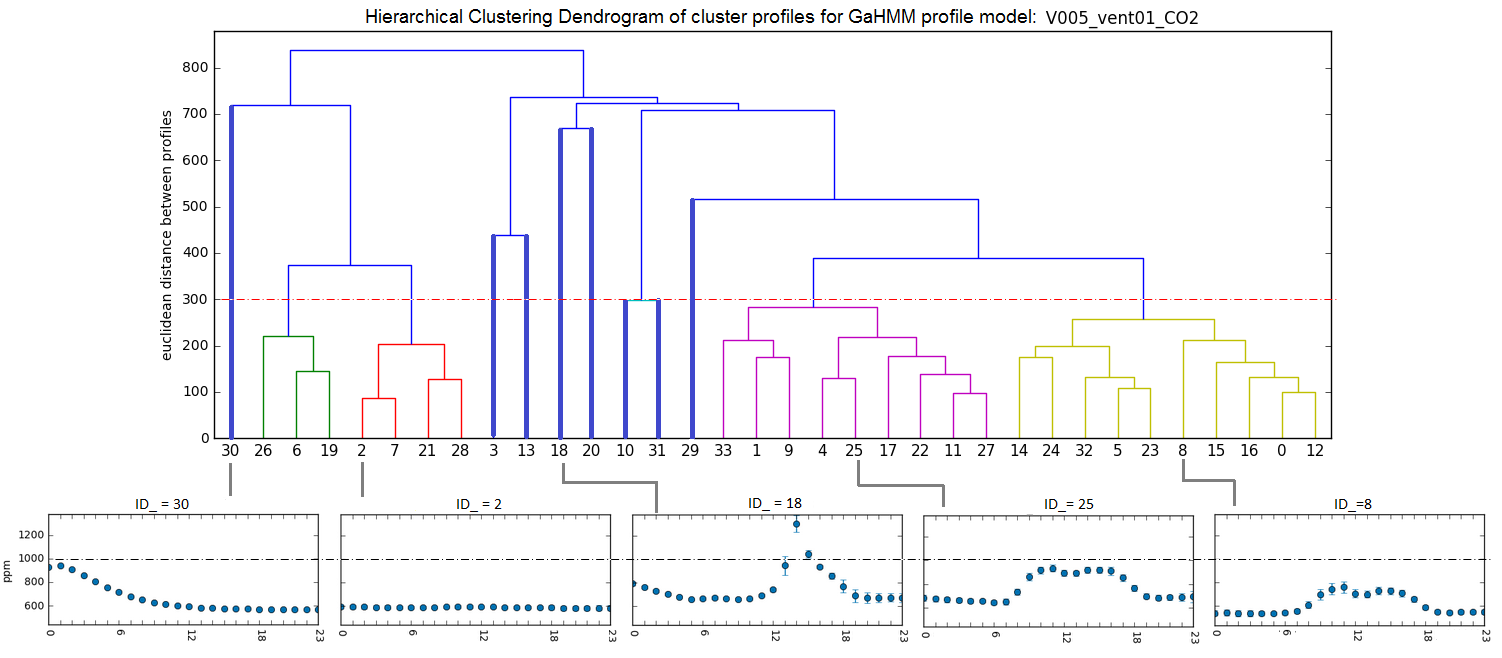
\includegraphics[scale=0.65]{Figures/dendrogram_CO2_NE_complete.jpg}
  \caption{Hierarchical clustering dendrogram for the $CO_2$ cluster profiles of the North-East part of the building.}
  \label{fig:dendrogram_CO2_NE_complete}
\end{figure}

\begin{figure}[h!]
  \vspace{0.5em} %better style
  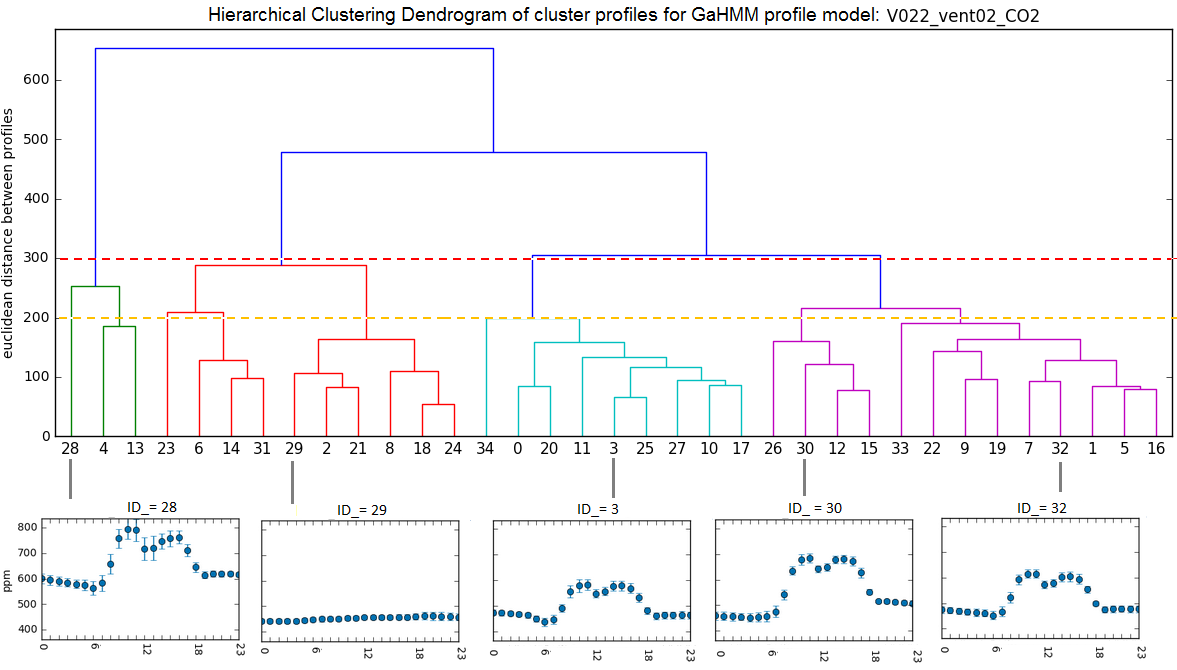
\includegraphics[scale=0.68]{Figures/dendrogram_CO2_SW_complete.jpg}
  \caption{Hierarchical clustering dendrogram for the $CO_2$ cluster profiles of the South-West part of the building.}
  \label{fig:dendrogram_CO2_SW_complete}
\end{figure}


\begin{figure}[h!]
  \vspace{0.5em} %better style
  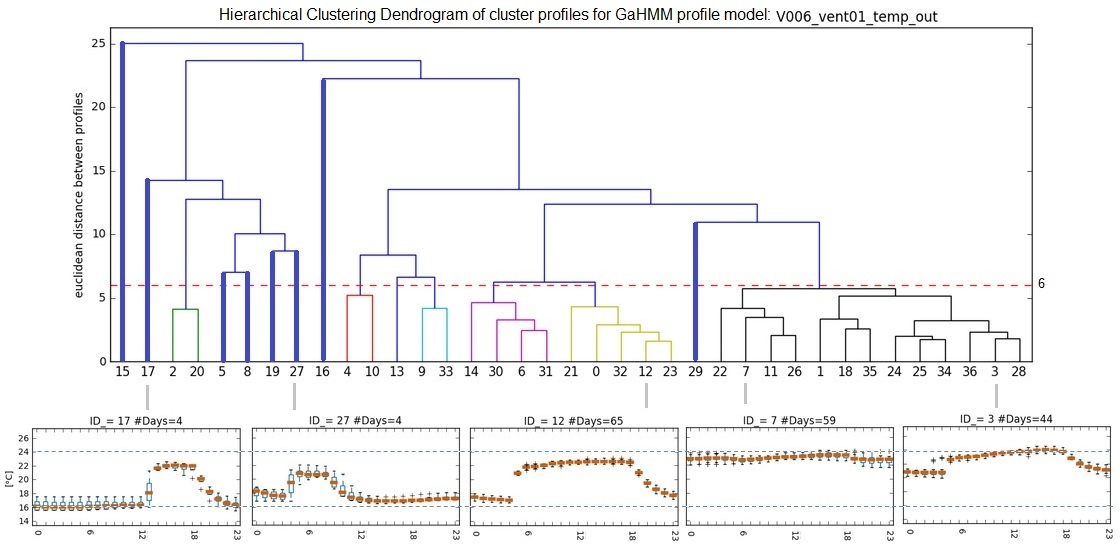
\includegraphics[scale=0.78]{Figures/dendogram_temperature_exhaust_air_NE.jpg}
  \caption{Hierarchical clustering dendrogram for \textit{exhausted air temperature - cluster profiles} of  
  the North-East ventilation system.}
  \label{fig:dendrogram_exhausted_NE}
\end{figure}

\begin{figure}[h!]
  \vspace{0.5em} %better style
  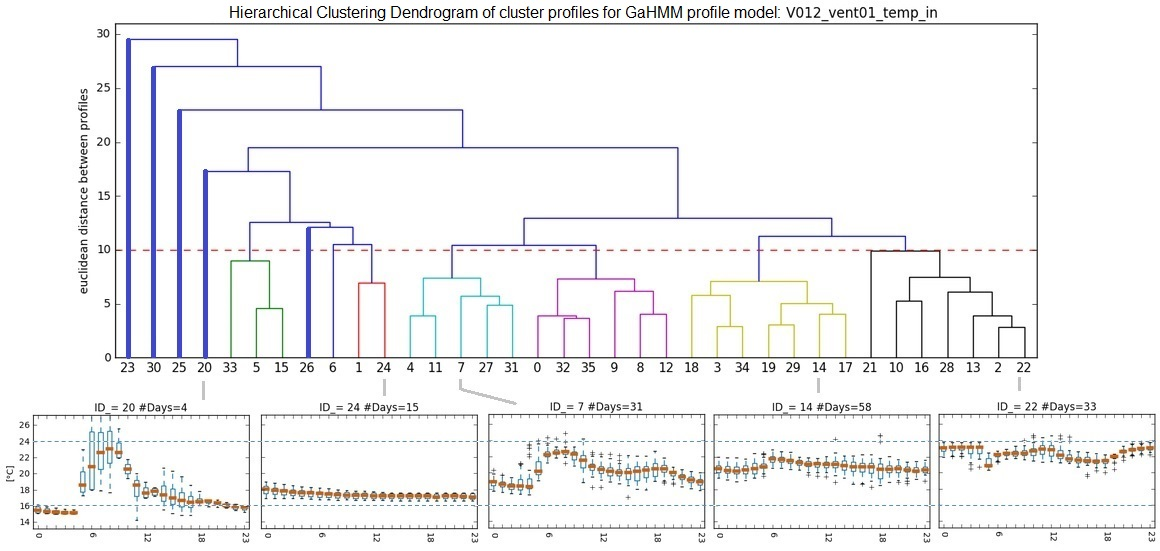
\includegraphics[scale=0.78]{Figures/Dendrogram_temperature_intake_NE.jpg}
  \caption{Hierarchical clustering dendrogram for \textit{intake air temperature - cluster profiles} of the North-East ventilation system.}
  \label{fig:dendrogram_intake_NE}
\end{figure}

\begin{figure}[h!]
  \vspace{0.5em} %better style
  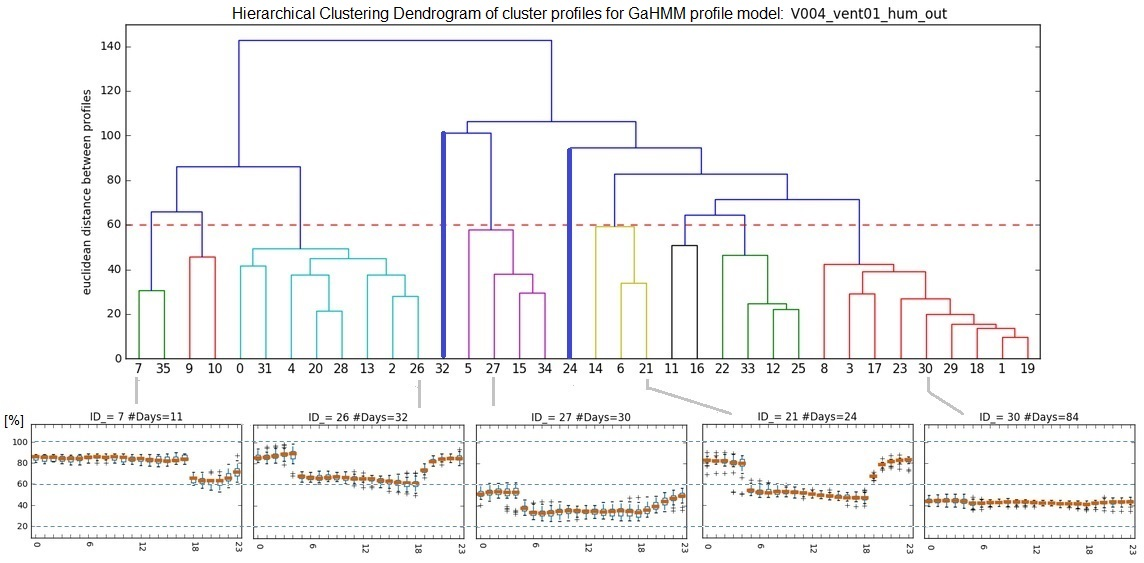
\includegraphics[scale=0.78]{Figures/dendrogram_humidity_out_NE.jpg}
  \caption{Hierarchical clustering dendrogram for \textit{exhausted air humidity - cluster profiles} of  
  the North-East ventilation system.}
  \label{fig:dendrogram_exhausted_humidity_NE}
\end{figure}

\begin{figure}[h!]
  \vspace{0.5em} %better style
  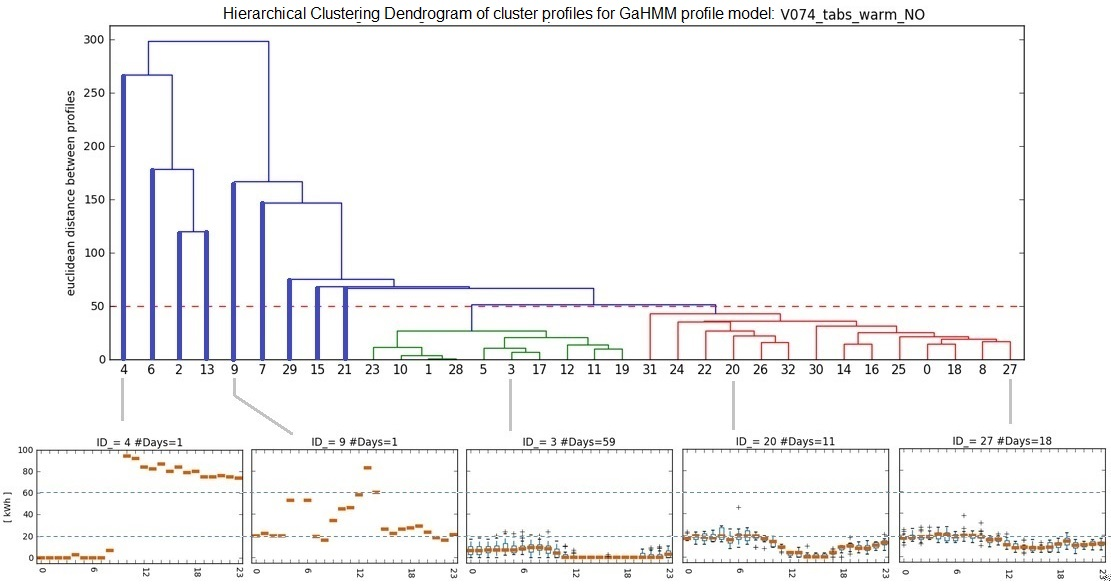
\includegraphics[scale=0.78]{Figures/dend_heating_NE_1.jpg}
  \caption{Hierarchical clustering dendrogram for \textit{heating consumption energy - cluster profiles} of the North-East part of the building.}
  \label{fig:dendrogram_heating_NE}
\end{figure}


\begin{figure}[h!]
  \vspace{0.5em} %better style
  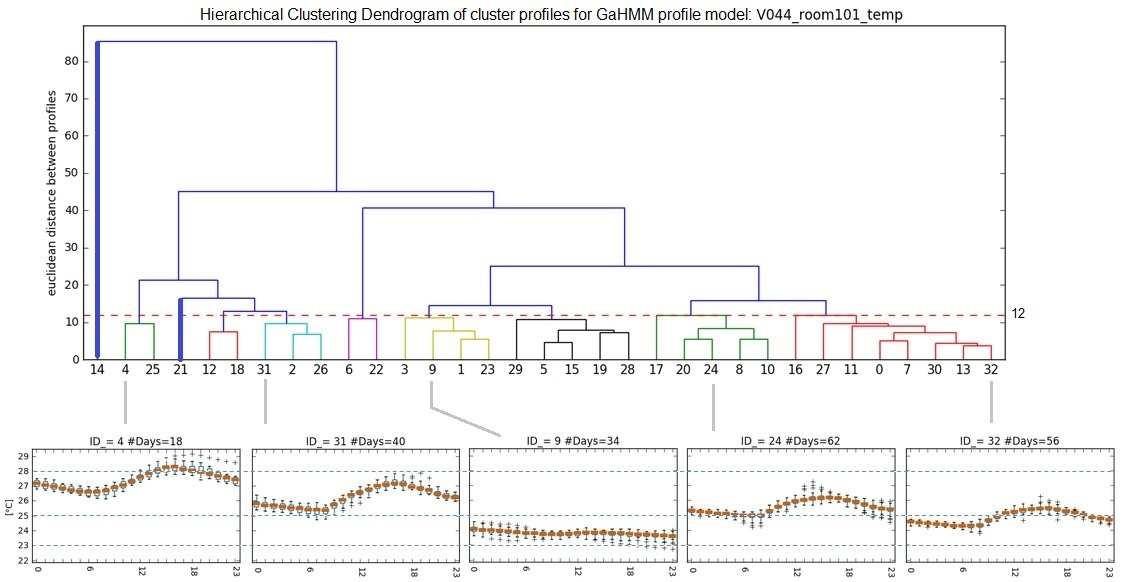
\includegraphics[scale=0.78]{Figures/Dendrogran_room_temperature_NE.jpg}
  \caption{Hierarchical clustering dendrogram for \textit{room temperature - cluster profiles} of room 101 that belongs to the North-East part of the building.}
  \label{fig:dendrogram_room_temperature_NE}
\end{figure}




\end{landscape}
\restoregeometry




  
% Table generated by Excel2LaTeX from sheet 'Discord_clusters'
\begin{table}[htbp]
  \centering
  \scriptsize
  \caption{Discord clusters profile of the CO2 level variable that belongs to the North-East zone of the building.}
    \begin{tabular}{|c|l|r|r|r|r|r|r|r|r|r|r|r|r|}
    \hline
    \rowcolor[rgb]{ .553,  .706,  .886} \multicolumn{2}{|c|}{\textbf{Profile code}} & \textbf{00:00} & \textbf{01:00} & \textbf{02:00} & \textbf{03:00} & \textbf{04:00} & \textbf{05:00} & \textbf{06:00} & \textbf{07:00} & \textbf{08:00} & \textbf{09:00} & \textbf{10:00} & \textbf{11:00} \bigstrut\\
    \hline
    \rowcolor[rgb]{ .553,  .706,  .886} \textbf{3} & \textbf{mean} & \cellcolor[rgb]{ 1,  1,  1} 705.9 & \cellcolor[rgb]{ 1,  1,  1} 682.5 & \cellcolor[rgb]{ 1,  1,  1} 662.2 & \cellcolor[rgb]{ 1,  1,  1} 643.8 & \cellcolor[rgb]{ 1,  1,  1} 629.7 & \cellcolor[rgb]{ 1,  1,  1} 624.4 & \cellcolor[rgb]{ 1,  1,  1} 625.4 & \cellcolor[rgb]{ 1,  1,  1} 641.6 & \cellcolor[rgb]{ 1,  1,  1} 672.0 & \cellcolor[rgb]{ 1,  1,  1} 710.1 & \cellcolor[rgb]{ 1,  1,  1} 711.9 & \cellcolor[rgb]{ 1,  1,  1} 714.6 \bigstrut\\
\cline{2-14}    \rowcolor[rgb]{ .553,  .706,  .886}      & \textbf{std} & \cellcolor[rgb]{ 1,  1,  1} 63.1 & \cellcolor[rgb]{ 1,  1,  1} 53.2 & \cellcolor[rgb]{ 1,  1,  1} 44.8 & \cellcolor[rgb]{ 1,  1,  1} 37.8 & \cellcolor[rgb]{ 1,  1,  1} 34.0 & \cellcolor[rgb]{ 1,  1,  1} 26.6 & \cellcolor[rgb]{ 1,  1,  1} 31.5 & \cellcolor[rgb]{ 1,  1,  1} 36.9 & \cellcolor[rgb]{ 1,  1,  1} 24.6 & \cellcolor[rgb]{ 1,  1,  1} 54.3 & \cellcolor[rgb]{ 1,  1,  1} 53.9 & \cellcolor[rgb]{ 1,  1,  1} 28.0 \bigstrut\\
    \hline
    \rowcolor[rgb]{ .553,  .706,  .886} \textbf{10} & \textbf{mean} & \cellcolor[rgb]{ .851,  .851,  .851} 701.2 & \cellcolor[rgb]{ .851,  .851,  .851} 692.3 & \cellcolor[rgb]{ .851,  .851,  .851} 683.9 & \cellcolor[rgb]{ .851,  .851,  .851} 675.4 & \cellcolor[rgb]{ .851,  .851,  .851} 670.6 & \cellcolor[rgb]{ .851,  .851,  .851} 682.6 & \cellcolor[rgb]{ .851,  .851,  .851} 665.2 & \cellcolor[rgb]{ .851,  .851,  .851} 667.1 & \cellcolor[rgb]{ .851,  .851,  .851} 748.5 & \cellcolor[rgb]{ .851,  .851,  .851} 878.1 & \cellcolor[rgb]{ .851,  .851,  .851} 956.8 & \cellcolor[rgb]{ .851,  .851,  .851} 991.6 \bigstrut\\
\cline{2-14}    \rowcolor[rgb]{ .553,  .706,  .886}      & \textbf{std} & \cellcolor[rgb]{ .851,  .851,  .851} 35.6 & \cellcolor[rgb]{ .851,  .851,  .851} 34.4 & \cellcolor[rgb]{ .851,  .851,  .851} 32.4 & \cellcolor[rgb]{ .851,  .851,  .851} 30.4 & \cellcolor[rgb]{ .851,  .851,  .851} 26.4 & \cellcolor[rgb]{ .851,  .851,  .851} 17.2 & \cellcolor[rgb]{ .851,  .851,  .851} 16.3 & \cellcolor[rgb]{ .851,  .851,  .851} 18.8 & \cellcolor[rgb]{ .851,  .851,  .851} 24.0 & \cellcolor[rgb]{ .851,  .851,  .851} 24.4 & \cellcolor[rgb]{ .851,  .851,  .851} 39.5 & \cellcolor[rgb]{ .851,  .851,  .851} 52.1 \bigstrut\\
    \hline
    \rowcolor[rgb]{ .553,  .706,  .886} \textbf{18} & \textbf{mean} & \cellcolor[rgb]{ 1,  1,  1} 790.1 & \cellcolor[rgb]{ 1,  1,  1} 758.1 & \cellcolor[rgb]{ 1,  1,  1} 727.7 & \cellcolor[rgb]{ 1,  1,  1} 699.7 & \cellcolor[rgb]{ 1,  1,  1} 677.3 & \cellcolor[rgb]{ 1,  1,  1} 657.4 & \cellcolor[rgb]{ 1,  1,  1} 660.5 & \cellcolor[rgb]{ 1,  1,  1} 670.0 & \cellcolor[rgb]{ 1,  1,  1} 665.2 & \cellcolor[rgb]{ 1,  1,  1} 657.8 & \cellcolor[rgb]{ 1,  1,  1} 660.8 & \cellcolor[rgb]{ 1,  1,  1} 691.1 \bigstrut\\
\cline{2-14}    \rowcolor[rgb]{ .553,  .706,  .886}      & \textbf{std} & \cellcolor[rgb]{ 1,  1,  1} 15.9 & \cellcolor[rgb]{ 1,  1,  1} 13.3 & \cellcolor[rgb]{ 1,  1,  1} 12.6 & \cellcolor[rgb]{ 1,  1,  1} 10.7 & \cellcolor[rgb]{ 1,  1,  1} 10.2 & \cellcolor[rgb]{ 1,  1,  1} 8.8 & \cellcolor[rgb]{ 1,  1,  1} 10.9 & \cellcolor[rgb]{ 1,  1,  1} 11.0 & \cellcolor[rgb]{ 1,  1,  1} 11.4 & \cellcolor[rgb]{ 1,  1,  1} 10.1 & \cellcolor[rgb]{ 1,  1,  1} 9.1 & \cellcolor[rgb]{ 1,  1,  1} 11.4 \bigstrut\\
    \hline
    \rowcolor[rgb]{ .553,  .706,  .886} \textbf{29} & \textbf{mean} & \cellcolor[rgb]{ .851,  .851,  .851} 843.8 & \cellcolor[rgb]{ .851,  .851,  .851} 831.1 & \cellcolor[rgb]{ .851,  .851,  .851} 813.1 & \cellcolor[rgb]{ .851,  .851,  .851} 792.2 & \cellcolor[rgb]{ .851,  .851,  .851} 771.8 & \cellcolor[rgb]{ .851,  .851,  .851} 644.8 & \cellcolor[rgb]{ .851,  .851,  .851} 603.8 & \cellcolor[rgb]{ .851,  .851,  .851} 605.8 & \cellcolor[rgb]{ .851,  .851,  .851} 681.9 & \cellcolor[rgb]{ .851,  .851,  .851} 776.9 & \cellcolor[rgb]{ .851,  .851,  .851} 849.2 & \cellcolor[rgb]{ .851,  .851,  .851} 888.9 \bigstrut\\
\cline{2-14}    \rowcolor[rgb]{ .553,  .706,  .886}      & \textbf{std} & \cellcolor[rgb]{ .851,  .851,  .851} 9.6 & \cellcolor[rgb]{ .851,  .851,  .851} 18.2 & \cellcolor[rgb]{ .851,  .851,  .851} 24.3 & \cellcolor[rgb]{ .851,  .851,  .851} 31.8 & \cellcolor[rgb]{ .851,  .851,  .851} 38.8 & \cellcolor[rgb]{ .851,  .851,  .851} 15.9 & \cellcolor[rgb]{ .851,  .851,  .851} 10.9 & \cellcolor[rgb]{ .851,  .851,  .851} 8.2 & \cellcolor[rgb]{ .851,  .851,  .851} 7.2 & \cellcolor[rgb]{ .851,  .851,  .851} 1.4 & \cellcolor[rgb]{ .851,  .851,  .851} 7.9 & \cellcolor[rgb]{ .851,  .851,  .851} 6.1 \bigstrut\\
    \hline
    \rowcolor[rgb]{ .553,  .706,  .886} \textbf{13} & \textbf{mean} & \cellcolor[rgb]{ 1,  1,  1} 537 & \cellcolor[rgb]{ 1,  1,  1} 536 & \cellcolor[rgb]{ 1,  1,  1} 534.3 & \cellcolor[rgb]{ 1,  1,  1} 531.2 & \cellcolor[rgb]{ 1,  1,  1} 532 & \cellcolor[rgb]{ 1,  1,  1} 532 & \cellcolor[rgb]{ 1,  1,  1} 533 & \cellcolor[rgb]{ 1,  1,  1} 537 & \cellcolor[rgb]{ 1,  1,  1} 559 & \cellcolor[rgb]{ 1,  1,  1} 566 & \cellcolor[rgb]{ 1,  1,  1} 580 & \cellcolor[rgb]{ 1,  1,  1} 615 \bigstrut\\
\cline{2-14}    \rowcolor[rgb]{ .553,  .706,  .886}      & \textbf{std} & \cellcolor[rgb]{ 1,  1,  1} 10.6 & \cellcolor[rgb]{ 1,  1,  1} 11 & \cellcolor[rgb]{ 1,  1,  1} 11.4 & \cellcolor[rgb]{ 1,  1,  1} 11.88 & \cellcolor[rgb]{ 1,  1,  1} 9.27 & \cellcolor[rgb]{ 1,  1,  1} 9.86 & \cellcolor[rgb]{ 1,  1,  1} 12.3 & \cellcolor[rgb]{ 1,  1,  1} 13.5 & \cellcolor[rgb]{ 1,  1,  1} 32.6 & \cellcolor[rgb]{ 1,  1,  1} 29.9 & \cellcolor[rgb]{ 1,  1,  1} 17 & \cellcolor[rgb]{ 1,  1,  1} 11.1 \bigstrut\\
    \hline
    \rowcolor[rgb]{ .553,  .706,  .886} \textbf{26} & \textbf{mean} & \cellcolor[rgb]{ .851,  .851,  .851} 719.1 & \cellcolor[rgb]{ .851,  .851,  .851} 712.1 & \cellcolor[rgb]{ .851,  .851,  .851} 703.6 & \cellcolor[rgb]{ .851,  .851,  .851} 694.6 & \cellcolor[rgb]{ .851,  .851,  .851} 685.5 & \cellcolor[rgb]{ .851,  .851,  .851} 676.0 & \cellcolor[rgb]{ .851,  .851,  .851} 670.0 & \cellcolor[rgb]{ .851,  .851,  .851} 667.0 & \cellcolor[rgb]{ .851,  .851,  .851} 663.9 & \cellcolor[rgb]{ .851,  .851,  .851} 661.0 & \cellcolor[rgb]{ .851,  .851,  .851} 658.5 & \cellcolor[rgb]{ .851,  .851,  .851} 655.3 \bigstrut\\
\cline{2-14}    \rowcolor[rgb]{ .553,  .706,  .886}      & \textbf{std} & \cellcolor[rgb]{ .851,  .851,  .851} 45.9 & \cellcolor[rgb]{ .851,  .851,  .851} 37.9 & \cellcolor[rgb]{ .851,  .851,  .851} 33.1 & \cellcolor[rgb]{ .851,  .851,  .851} 30.7 & \cellcolor[rgb]{ .851,  .851,  .851} 30.0 & \cellcolor[rgb]{ .851,  .851,  .851} 30.6 & \cellcolor[rgb]{ .851,  .851,  .851} 31.3 & \cellcolor[rgb]{ .851,  .851,  .851} 31.3 & \cellcolor[rgb]{ .851,  .851,  .851} 32.9 & \cellcolor[rgb]{ .851,  .851,  .851} 34.6 & \cellcolor[rgb]{ .851,  .851,  .851} 37.9 & \cellcolor[rgb]{ .851,  .851,  .851} 40.0 \bigstrut\\
    \hline
    \rowcolor[rgb]{ .553,  .706,  .886} \textbf{20} & \textbf{mean} & \cellcolor[rgb]{ 1,  1,  1} 551 & \cellcolor[rgb]{ 1,  1,  1} 549 & \cellcolor[rgb]{ 1,  1,  1} 549 & \cellcolor[rgb]{ 1,  1,  1} 545.1 & \cellcolor[rgb]{ 1,  1,  1} 544 & \cellcolor[rgb]{ 1,  1,  1} 542 & \cellcolor[rgb]{ 1,  1,  1} 542 & \cellcolor[rgb]{ 1,  1,  1} 541 & \cellcolor[rgb]{ 1,  1,  1} 542 & \cellcolor[rgb]{ 1,  1,  1} 549 & \cellcolor[rgb]{ 1,  1,  1} 564 & \cellcolor[rgb]{ 1,  1,  1} 600 \bigstrut\\
\cline{2-14}    \rowcolor[rgb]{ .553,  .706,  .886}      & \textbf{std} & \cellcolor[rgb]{ 1,  1,  1} 0.1 & \cellcolor[rgb]{ 1,  1,  1} 0.1 & \cellcolor[rgb]{ 1,  1,  1} 0.1 & \cellcolor[rgb]{ 1,  1,  1} 0.1 & \cellcolor[rgb]{ 1,  1,  1} 0.1 & \cellcolor[rgb]{ 1,  1,  1} 0.1 & \cellcolor[rgb]{ 1,  1,  1} 0.1 & \cellcolor[rgb]{ 1,  1,  1} 0.1 & \cellcolor[rgb]{ 1,  1,  1} 0.1 & \cellcolor[rgb]{ 1,  1,  1} 0.1 & \cellcolor[rgb]{ 1,  1,  1} 0.1 & \cellcolor[rgb]{ 1,  1,  1} 0.1 \bigstrut\\
    \hline
    \rowcolor[rgb]{ .553,  .706,  .886} \textbf{30} & \textbf{mean} & \cellcolor[rgb]{ .851,  .851,  .851} 930.8 & \cellcolor[rgb]{ .851,  .851,  .851} 942.8 & \cellcolor[rgb]{ .851,  .851,  .851} 908.5 & \cellcolor[rgb]{ .851,  .851,  .851} 859.1 & \cellcolor[rgb]{ .851,  .851,  .851} 805.4 & \cellcolor[rgb]{ .851,  .851,  .851} 758.0 & \cellcolor[rgb]{ .851,  .851,  .851} 718.0 & \cellcolor[rgb]{ .851,  .851,  .851} 681.0 & \cellcolor[rgb]{ .851,  .851,  .851} 652.7 & \cellcolor[rgb]{ .851,  .851,  .851} 629.8 & \cellcolor[rgb]{ .851,  .851,  .851} 613.9 & \cellcolor[rgb]{ .851,  .851,  .851} 601.6 \bigstrut\\
\cline{2-14}    \rowcolor[rgb]{ .553,  .706,  .886}      & \textbf{std} & \cellcolor[rgb]{ .851,  .851,  .851} 0.1 & \cellcolor[rgb]{ .851,  .851,  .851} 0.1 & \cellcolor[rgb]{ .851,  .851,  .851} 0.1 & \cellcolor[rgb]{ .851,  .851,  .851} 0.1 & \cellcolor[rgb]{ .851,  .851,  .851} 0.1 & \cellcolor[rgb]{ .851,  .851,  .851} 0.1 & \cellcolor[rgb]{ .851,  .851,  .851} 0.1 & \cellcolor[rgb]{ .851,  .851,  .851} 0.1 & \cellcolor[rgb]{ .851,  .851,  .851} 0.1 & \cellcolor[rgb]{ .851,  .851,  .851} 0.1 & \cellcolor[rgb]{ .851,  .851,  .851} 0.1 & \cellcolor[rgb]{ .851,  .851,  .851} 0.1 \bigstrut\\
    \hline
    \rowcolor[rgb]{ .553,  .706,  .886} \textbf{31} & \textbf{mean} & \cellcolor[rgb]{ 1,  1,  1} 819 & \cellcolor[rgb]{ 1,  1,  1} 806 & \cellcolor[rgb]{ 1,  1,  1} 788.4 & \cellcolor[rgb]{ 1,  1,  1} 772.2 & \cellcolor[rgb]{ 1,  1,  1} 756 & \cellcolor[rgb]{ 1,  1,  1} 748 & \cellcolor[rgb]{ 1,  1,  1} 722 & \cellcolor[rgb]{ 1,  1,  1} 727 & \cellcolor[rgb]{ 1,  1,  1} 803 & \cellcolor[rgb]{ 1,  1,  1} 928 & \cellcolor[rgb]{ 1,  1,  1} 996 & \cellcolor[rgb]{ 1,  1,  1} 1025 \bigstrut\\
\cline{2-14}    \rowcolor[rgb]{ .553,  .706,  .886}      & \textbf{std} & \cellcolor[rgb]{ 1,  1,  1} 21.3 & \cellcolor[rgb]{ 1,  1,  1} 22.8 & \cellcolor[rgb]{ 1,  1,  1} 21.58 & \cellcolor[rgb]{ 1,  1,  1} 20.24 & \cellcolor[rgb]{ 1,  1,  1} 18.9 & \cellcolor[rgb]{ 1,  1,  1} 17.7 & \cellcolor[rgb]{ 1,  1,  1} 25.6 & \cellcolor[rgb]{ 1,  1,  1} 28.7 & \cellcolor[rgb]{ 1,  1,  1} 30.9 & \cellcolor[rgb]{ 1,  1,  1} 35.9 & \cellcolor[rgb]{ 1,  1,  1} 30.2 & \cellcolor[rgb]{ 1,  1,  1} 20.7 \bigstrut\\
    \hline
    \rowcolor[rgb]{ .553,  .706,  .886} \textbf{33} & \textbf{mean} & \cellcolor[rgb]{ .851,  .851,  .851} 702.7 & \cellcolor[rgb]{ .851,  .851,  .851} 699.8 & \cellcolor[rgb]{ .851,  .851,  .851} 695.1 & \cellcolor[rgb]{ .851,  .851,  .851} 689.6 & \cellcolor[rgb]{ .851,  .851,  .851} 683.3 & \cellcolor[rgb]{ .851,  .851,  .851} 660.3 & \cellcolor[rgb]{ .851,  .851,  .851} 645.8 & \cellcolor[rgb]{ .851,  .851,  .851} 650.1 & \cellcolor[rgb]{ .851,  .851,  .851} 705.2 & \cellcolor[rgb]{ .851,  .851,  .851} 791.3 & \cellcolor[rgb]{ .851,  .851,  .851} 835.3 & \cellcolor[rgb]{ .851,  .851,  .851} 842.7 \bigstrut\\
\cline{2-14}    \rowcolor[rgb]{ .553,  .706,  .886}      & \textbf{std} & \cellcolor[rgb]{ .851,  .851,  .851} 23.3 & \cellcolor[rgb]{ .851,  .851,  .851} 22.2 & \cellcolor[rgb]{ .851,  .851,  .851} 21.2 & \cellcolor[rgb]{ .851,  .851,  .851} 20.1 & \cellcolor[rgb]{ .851,  .851,  .851} 18.9 & \cellcolor[rgb]{ .851,  .851,  .851} 28.6 & \cellcolor[rgb]{ .851,  .851,  .851} 26.0 & \cellcolor[rgb]{ .851,  .851,  .851} 22.4 & \cellcolor[rgb]{ .851,  .851,  .851} 35.3 & \cellcolor[rgb]{ .851,  .851,  .851} 40.2 & \cellcolor[rgb]{ .851,  .851,  .851} 24.9 & \cellcolor[rgb]{ .851,  .851,  .851} 23.8 \bigstrut\\
    \hline
    \rowcolor[rgb]{ .553,  .706,  .886} \textbf{4} & \textbf{mean} & \cellcolor[rgb]{ 1,  1,  1} 664 & \cellcolor[rgb]{ 1,  1,  1} 654 & \cellcolor[rgb]{ 1,  1,  1} 644.7 & \cellcolor[rgb]{ 1,  1,  1} 634.8 & \cellcolor[rgb]{ 1,  1,  1} 625 & \cellcolor[rgb]{ 1,  1,  1} 627 & \cellcolor[rgb]{ 1,  1,  1} 596 & \cellcolor[rgb]{ 1,  1,  1} 597 & \cellcolor[rgb]{ 1,  1,  1} 681 & \cellcolor[rgb]{ 1,  1,  1} 826 & \cellcolor[rgb]{ 1,  1,  1} 905 & \cellcolor[rgb]{ 1,  1,  1} 939 \bigstrut\\
\cline{2-14}    \rowcolor[rgb]{ .553,  .706,  .886}      & \textbf{std} & \cellcolor[rgb]{ 1,  1,  1} 19.5 & \cellcolor[rgb]{ 1,  1,  1} 17.4 & \cellcolor[rgb]{ 1,  1,  1} 15.65 & \cellcolor[rgb]{ 1,  1,  1} 13.52 & \cellcolor[rgb]{ 1,  1,  1} 13.5 & \cellcolor[rgb]{ 1,  1,  1} 19.6 & \cellcolor[rgb]{ 1,  1,  1} 11.1 & \cellcolor[rgb]{ 1,  1,  1} 10.7 & \cellcolor[rgb]{ 1,  1,  1} 23.3 & \cellcolor[rgb]{ 1,  1,  1} 22.7 & \cellcolor[rgb]{ 1,  1,  1} 20.7 & \cellcolor[rgb]{ 1,  1,  1} 27.5 \bigstrut\\
    \hline
    \multicolumn{1}{r}{} & \multicolumn{1}{r}{} & \multicolumn{1}{r}{} & \multicolumn{1}{r}{} & \multicolumn{1}{r}{} & \multicolumn{1}{r}{} & \multicolumn{1}{r}{} & \multicolumn{1}{r}{} & \multicolumn{1}{r}{} & \multicolumn{1}{r}{} & \multicolumn{1}{r}{} & \multicolumn{1}{r}{} & \multicolumn{1}{r}{} & \multicolumn{1}{r}{} \bigstrut\\
    \hline
    \rowcolor[rgb]{ .553,  .706,  .886} \multicolumn{2}{|c|}{\textbf{Profile code}} & \textbf{12:00} & \textbf{13:00} & \textbf{14:00} & \textbf{15:00} & \textbf{16:00} & \textbf{17:00} & \textbf{18:00} & \textbf{19:00} & \textbf{20:00} & \textbf{21:00} & \textbf{22:00} & \textbf{23:00} \bigstrut\\
    \hline
    \rowcolor[rgb]{ .553,  .706,  .886} \textbf{3} & \textbf{mean} & \cellcolor[rgb]{ 1,  1,  1} 742.2 & \cellcolor[rgb]{ 1,  1,  1} 782.2 & \cellcolor[rgb]{ 1,  1,  1} 817.1 & \cellcolor[rgb]{ 1,  1,  1} 849.3 & \cellcolor[rgb]{ 1,  1,  1} 876.9 & \cellcolor[rgb]{ 1,  1,  1} 895.0 & \cellcolor[rgb]{ 1,  1,  1} 903.6 & \cellcolor[rgb]{ 1,  1,  1} 900.8 & \cellcolor[rgb]{ 1,  1,  1} 889.0 & \cellcolor[rgb]{ 1,  1,  1} 869.8 & \cellcolor[rgb]{ 1,  1,  1} 836.9 & \cellcolor[rgb]{ 1,  1,  1} 800.4 \bigstrut\\
\cline{2-14}    \rowcolor[rgb]{ .553,  .706,  .886}      & \textbf{std} & \cellcolor[rgb]{ 1,  1,  1} 31.3 & \cellcolor[rgb]{ 1,  1,  1} 40.4 & \cellcolor[rgb]{ 1,  1,  1} 44.3 & \cellcolor[rgb]{ 1,  1,  1} 43.1 & \cellcolor[rgb]{ 1,  1,  1} 43.1 & \cellcolor[rgb]{ 1,  1,  1} 42.9 & \cellcolor[rgb]{ 1,  1,  1} 40.1 & \cellcolor[rgb]{ 1,  1,  1} 36.9 & \cellcolor[rgb]{ 1,  1,  1} 36.0 & \cellcolor[rgb]{ 1,  1,  1} 34.8 & \cellcolor[rgb]{ 1,  1,  1} 32.9 & \cellcolor[rgb]{ 1,  1,  1} 32.5 \bigstrut\\
    \hline
    \rowcolor[rgb]{ .553,  .706,  .886} \textbf{10} & \textbf{mean} & \cellcolor[rgb]{ .851,  .851,  .851} 956.8 & \cellcolor[rgb]{ .851,  .851,  .851} 949.9 & \cellcolor[rgb]{ .851,  .851,  .851} 973.9 & \cellcolor[rgb]{ .851,  .851,  .851} 972.0 & \cellcolor[rgb]{ .851,  .851,  .851} 969.4 & \cellcolor[rgb]{ .851,  .851,  .851} 922.7 & \cellcolor[rgb]{ .851,  .851,  .851} 830.1 & \cellcolor[rgb]{ .851,  .851,  .851} 756.2 & \cellcolor[rgb]{ .851,  .851,  .851} 742.9 & \cellcolor[rgb]{ .851,  .851,  .851} 754.7 & \cellcolor[rgb]{ .851,  .851,  .851} 760.6 & \cellcolor[rgb]{ .851,  .851,  .851} 756.5 \bigstrut\\
\cline{2-14}    \rowcolor[rgb]{ .553,  .706,  .886}      & \textbf{std} & \cellcolor[rgb]{ .851,  .851,  .851} 51.6 & \cellcolor[rgb]{ .851,  .851,  .851} 34.5 & \cellcolor[rgb]{ .851,  .851,  .851} 33.8 & \cellcolor[rgb]{ .851,  .851,  .851} 37.8 & \cellcolor[rgb]{ .851,  .851,  .851} 40.1 & \cellcolor[rgb]{ .851,  .851,  .851} 36.2 & \cellcolor[rgb]{ .851,  .851,  .851} 35.4 & \cellcolor[rgb]{ .851,  .851,  .851} 32.8 & \cellcolor[rgb]{ .851,  .851,  .851} 28.4 & \cellcolor[rgb]{ .851,  .851,  .851} 36.9 & \cellcolor[rgb]{ .851,  .851,  .851} 49.0 & \cellcolor[rgb]{ .851,  .851,  .851} 55.8 \bigstrut\\
    \hline
    \rowcolor[rgb]{ .553,  .706,  .886} \textbf{18} & \textbf{mean} & \cellcolor[rgb]{ 1,  1,  1} 739.1 & \cellcolor[rgb]{ 1,  1,  1} 945.1 & \cellcolor[rgb]{ 1,  1,  1} 1301.5 & \cellcolor[rgb]{ 1,  1,  1} 1044.4 & \cellcolor[rgb]{ 1,  1,  1} 933.7 & \cellcolor[rgb]{ 1,  1,  1} 855.7 & \cellcolor[rgb]{ 1,  1,  1} 767.3 & \cellcolor[rgb]{ 1,  1,  1} 686.4 & \cellcolor[rgb]{ 1,  1,  1} 668.0 & \cellcolor[rgb]{ 1,  1,  1} 667.9 & \cellcolor[rgb]{ 1,  1,  1} 671.3 & \cellcolor[rgb]{ 1,  1,  1} 668.1 \bigstrut\\
\cline{2-14}    \rowcolor[rgb]{ .553,  .706,  .886}      & \textbf{std} & \cellcolor[rgb]{ 1,  1,  1} 15.8 & \cellcolor[rgb]{ 1,  1,  1} 79.0 & \cellcolor[rgb]{ 1,  1,  1} 73.7 & \cellcolor[rgb]{ 1,  1,  1} 33.7 & \cellcolor[rgb]{ 1,  1,  1} 14.2 & \cellcolor[rgb]{ 1,  1,  1} 23.6 & \cellcolor[rgb]{ 1,  1,  1} 54.9 & \cellcolor[rgb]{ 1,  1,  1} 56.2 & \cellcolor[rgb]{ 1,  1,  1} 44.6 & \cellcolor[rgb]{ 1,  1,  1} 39.6 & \cellcolor[rgb]{ 1,  1,  1} 36.3 & \cellcolor[rgb]{ 1,  1,  1} 37.7 \bigstrut\\
    \hline
    \rowcolor[rgb]{ .553,  .706,  .886} \textbf{29} & \textbf{mean} & \cellcolor[rgb]{ .851,  .851,  .851} 859.1 & \cellcolor[rgb]{ .851,  .851,  .851} 854.1 & \cellcolor[rgb]{ .851,  .851,  .851} 894.2 & \cellcolor[rgb]{ .851,  .851,  .851} 890.1 & \cellcolor[rgb]{ .851,  .851,  .851} 853.6 & \cellcolor[rgb]{ .851,  .851,  .851} 787.3 & \cellcolor[rgb]{ .851,  .851,  .851} 709.7 & \cellcolor[rgb]{ .851,  .851,  .851} 659.2 & \cellcolor[rgb]{ .851,  .851,  .851} 646.2 & \cellcolor[rgb]{ .851,  .851,  .851} 644.8 & \cellcolor[rgb]{ .851,  .851,  .851} 645.3 & \cellcolor[rgb]{ .851,  .851,  .851} 642.9 \bigstrut\\
\cline{2-14}    \rowcolor[rgb]{ .553,  .706,  .886}      & \textbf{std} & \cellcolor[rgb]{ .851,  .851,  .851} 8.1 & \cellcolor[rgb]{ .851,  .851,  .851} 13.9 & \cellcolor[rgb]{ .851,  .851,  .851} 17.4 & \cellcolor[rgb]{ .851,  .851,  .851} 29.6 & \cellcolor[rgb]{ .851,  .851,  .851} 43.6 & \cellcolor[rgb]{ .851,  .851,  .851} 33.8 & \cellcolor[rgb]{ .851,  .851,  .851} 6.0 & \cellcolor[rgb]{ .851,  .851,  .851} 11.3 & \cellcolor[rgb]{ .851,  .851,  .851} 13.6 & \cellcolor[rgb]{ .851,  .851,  .851} 13.8 & \cellcolor[rgb]{ .851,  .851,  .851} 16.5 & \cellcolor[rgb]{ .851,  .851,  .851} 18.8 \bigstrut\\
    \hline
    \rowcolor[rgb]{ .553,  .706,  .886} \textbf{13} & \textbf{mean} & \cellcolor[rgb]{ 1,  1,  1} 664 & \cellcolor[rgb]{ 1,  1,  1} 720 & \cellcolor[rgb]{ 1,  1,  1} 768.9 & \cellcolor[rgb]{ 1,  1,  1} 811.3 & \cellcolor[rgb]{ 1,  1,  1} 859 & \cellcolor[rgb]{ 1,  1,  1} 886 & \cellcolor[rgb]{ 1,  1,  1} 893 & \cellcolor[rgb]{ 1,  1,  1} 889 & \cellcolor[rgb]{ 1,  1,  1} 880 & \cellcolor[rgb]{ 1,  1,  1} 865 & \cellcolor[rgb]{ 1,  1,  1} 836 & \cellcolor[rgb]{ 1,  1,  1} 804 \bigstrut\\
\cline{2-14}    \rowcolor[rgb]{ .553,  .706,  .886}      & \textbf{std} & \cellcolor[rgb]{ 1,  1,  1} 13.5 & \cellcolor[rgb]{ 1,  1,  1} 12.8 & \cellcolor[rgb]{ 1,  1,  1} 13.13 & \cellcolor[rgb]{ 1,  1,  1} 21.64 & \cellcolor[rgb]{ 1,  1,  1} 7.64 & \cellcolor[rgb]{ 1,  1,  1} 26.6 & \cellcolor[rgb]{ 1,  1,  1} 42 & \cellcolor[rgb]{ 1,  1,  1} 48.8 & \cellcolor[rgb]{ 1,  1,  1} 51.3 & \cellcolor[rgb]{ 1,  1,  1} 48.7 & \cellcolor[rgb]{ 1,  1,  1} 41.5 & \cellcolor[rgb]{ 1,  1,  1} 35 \bigstrut\\
    \hline
    \rowcolor[rgb]{ .553,  .706,  .886} \textbf{26} & \textbf{mean} & \cellcolor[rgb]{ .851,  .851,  .851} 650.6 & \cellcolor[rgb]{ .851,  .851,  .851} 646.4 & \cellcolor[rgb]{ .851,  .851,  .851} 639.0 & \cellcolor[rgb]{ .851,  .851,  .851} 631.9 & \cellcolor[rgb]{ .851,  .851,  .851} 625.5 & \cellcolor[rgb]{ .851,  .851,  .851} 619.7 & \cellcolor[rgb]{ .851,  .851,  .851} 615.7 & \cellcolor[rgb]{ .851,  .851,  .851} 613.0 & \cellcolor[rgb]{ .851,  .851,  .851} 611.0 & \cellcolor[rgb]{ .851,  .851,  .851} 609.9 & \cellcolor[rgb]{ .851,  .851,  .851} 606.2 & \cellcolor[rgb]{ .851,  .851,  .851} 603.4 \bigstrut\\
\cline{2-14}    \rowcolor[rgb]{ .553,  .706,  .886}      & \textbf{std} & \cellcolor[rgb]{ .851,  .851,  .851} 40.9 & \cellcolor[rgb]{ .851,  .851,  .851} 40.3 & \cellcolor[rgb]{ .851,  .851,  .851} 36.5 & \cellcolor[rgb]{ .851,  .851,  .851} 35.1 & \cellcolor[rgb]{ .851,  .851,  .851} 34.2 & \cellcolor[rgb]{ .851,  .851,  .851} 34.1 & \cellcolor[rgb]{ .851,  .851,  .851} 33.8 & \cellcolor[rgb]{ .851,  .851,  .851} 35.6 & \cellcolor[rgb]{ .851,  .851,  .851} 35.7 & \cellcolor[rgb]{ .851,  .851,  .851} 36.5 & \cellcolor[rgb]{ .851,  .851,  .851} 37.6 & \cellcolor[rgb]{ .851,  .851,  .851} 38.6 \bigstrut\\
    \hline
    \rowcolor[rgb]{ .553,  .706,  .886} \textbf{20} & \textbf{mean} & \cellcolor[rgb]{ 1,  1,  1} 676 & \cellcolor[rgb]{ 1,  1,  1} 1167 & \cellcolor[rgb]{ 1,  1,  1} 973.4 & \cellcolor[rgb]{ 1,  1,  1} 902.5 & \cellcolor[rgb]{ 1,  1,  1} 883 & \cellcolor[rgb]{ 1,  1,  1} 839 & \cellcolor[rgb]{ 1,  1,  1} 737 & \cellcolor[rgb]{ 1,  1,  1} 661 & \cellcolor[rgb]{ 1,  1,  1} 648 & \cellcolor[rgb]{ 1,  1,  1} 656 & \cellcolor[rgb]{ 1,  1,  1} 662 & \cellcolor[rgb]{ 1,  1,  1} 658 \bigstrut\\
\cline{2-14}    \rowcolor[rgb]{ .553,  .706,  .886}      & \textbf{std} & \cellcolor[rgb]{ 1,  1,  1} 0.1 & \cellcolor[rgb]{ 1,  1,  1} 0.1 & \cellcolor[rgb]{ 1,  1,  1} 0.1 & \cellcolor[rgb]{ 1,  1,  1} 0.1 & \cellcolor[rgb]{ 1,  1,  1} 0.1 & \cellcolor[rgb]{ 1,  1,  1} 0.1 & \cellcolor[rgb]{ 1,  1,  1} 0.1 & \cellcolor[rgb]{ 1,  1,  1} 0.1 & \cellcolor[rgb]{ 1,  1,  1} 0.1 & \cellcolor[rgb]{ 1,  1,  1} 0.1 & \cellcolor[rgb]{ 1,  1,  1} 0.1 & \cellcolor[rgb]{ 1,  1,  1} 0.1 \bigstrut\\
    \hline
    \rowcolor[rgb]{ .553,  .706,  .886} \textbf{30} & \textbf{mean} & \cellcolor[rgb]{ .851,  .851,  .851} 592.2 & \cellcolor[rgb]{ .851,  .851,  .851} 585.0 & \cellcolor[rgb]{ .851,  .851,  .851} 580.8 & \cellcolor[rgb]{ .851,  .851,  .851} 577.1 & \cellcolor[rgb]{ .851,  .851,  .851} 574.0 & \cellcolor[rgb]{ .851,  .851,  .851} 573.1 & \cellcolor[rgb]{ .851,  .851,  .851} 568.5 & \cellcolor[rgb]{ .851,  .851,  .851} 566.5 & \cellcolor[rgb]{ .851,  .851,  .851} 570.5 & \cellcolor[rgb]{ .851,  .851,  .851} 570.2 & \cellcolor[rgb]{ .851,  .851,  .851} 567.9 & \cellcolor[rgb]{ .851,  .851,  .851} 566.5 \bigstrut\\
\cline{2-14}    \rowcolor[rgb]{ .553,  .706,  .886}      & \textbf{std} & \cellcolor[rgb]{ .851,  .851,  .851} 0.1 & \cellcolor[rgb]{ .851,  .851,  .851} 0.1 & \cellcolor[rgb]{ .851,  .851,  .851} 0.1 & \cellcolor[rgb]{ .851,  .851,  .851} 0.1 & \cellcolor[rgb]{ .851,  .851,  .851} 0.1 & \cellcolor[rgb]{ .851,  .851,  .851} 0.1 & \cellcolor[rgb]{ .851,  .851,  .851} 0.1 & \cellcolor[rgb]{ .851,  .851,  .851} 0.1 & \cellcolor[rgb]{ .851,  .851,  .851} 0.1 & \cellcolor[rgb]{ .851,  .851,  .851} 0.1 & \cellcolor[rgb]{ .851,  .851,  .851} 0.1 & \cellcolor[rgb]{ .851,  .851,  .851} 0.1 \bigstrut\\
    \hline
    \rowcolor[rgb]{ .553,  .706,  .886} \textbf{31} & \textbf{mean} & \cellcolor[rgb]{ 1,  1,  1} 988 & \cellcolor[rgb]{ 1,  1,  1} 971 & \cellcolor[rgb]{ 1,  1,  1} 1001 & \cellcolor[rgb]{ 1,  1,  1} 1024 & \cellcolor[rgb]{ 1,  1,  1} 1013 & \cellcolor[rgb]{ 1,  1,  1} 953 & \cellcolor[rgb]{ 1,  1,  1} 862 & \cellcolor[rgb]{ 1,  1,  1} 794 & \cellcolor[rgb]{ 1,  1,  1} 777 & \cellcolor[rgb]{ 1,  1,  1} 788 & \cellcolor[rgb]{ 1,  1,  1} 798 & \cellcolor[rgb]{ 1,  1,  1} 796 \bigstrut\\
\cline{2-14}    \rowcolor[rgb]{ .553,  .706,  .886}      & \textbf{std} & \cellcolor[rgb]{ 1,  1,  1} 15.9 & \cellcolor[rgb]{ 1,  1,  1} 47.7 & \cellcolor[rgb]{ 1,  1,  1} 37.59 & \cellcolor[rgb]{ 1,  1,  1} 30.83 & \cellcolor[rgb]{ 1,  1,  1} 21.2 & \cellcolor[rgb]{ 1,  1,  1} 28.4 & \cellcolor[rgb]{ 1,  1,  1} 29.3 & \cellcolor[rgb]{ 1,  1,  1} 26.3 & \cellcolor[rgb]{ 1,  1,  1} 25.2 & \cellcolor[rgb]{ 1,  1,  1} 31.5 & \cellcolor[rgb]{ 1,  1,  1} 40.3 & \cellcolor[rgb]{ 1,  1,  1} 46 \bigstrut\\
    \hline
    \rowcolor[rgb]{ .553,  .706,  .886} \textbf{33} & \textbf{mean} & \cellcolor[rgb]{ .851,  .851,  .851} 805.2 & \cellcolor[rgb]{ .851,  .851,  .851} 810.6 & \cellcolor[rgb]{ .851,  .851,  .851} 838.3 & \cellcolor[rgb]{ .851,  .851,  .851} 842.9 & \cellcolor[rgb]{ .851,  .851,  .851} 840.0 & \cellcolor[rgb]{ .851,  .851,  .851} 794.6 & \cellcolor[rgb]{ .851,  .851,  .851} 725.5 & \cellcolor[rgb]{ .851,  .851,  .851} 686.4 & \cellcolor[rgb]{ .851,  .851,  .851} 680.5 & \cellcolor[rgb]{ .851,  .851,  .851} 680.9 & \cellcolor[rgb]{ .851,  .851,  .851} 679.3 & \cellcolor[rgb]{ .851,  .851,  .851} 677.2 \bigstrut\\
\cline{2-14}    \rowcolor[rgb]{ .553,  .706,  .886}      & \textbf{std} & \cellcolor[rgb]{ .851,  .851,  .851} 21.8 & \cellcolor[rgb]{ .851,  .851,  .851} 22.6 & \cellcolor[rgb]{ .851,  .851,  .851} 32.8 & \cellcolor[rgb]{ .851,  .851,  .851} 29.0 & \cellcolor[rgb]{ .851,  .851,  .851} 25.6 & \cellcolor[rgb]{ .851,  .851,  .851} 15.7 & \cellcolor[rgb]{ .851,  .851,  .851} 14.2 & \cellcolor[rgb]{ .851,  .851,  .851} 15.1 & \cellcolor[rgb]{ .851,  .851,  .851} 15.8 & \cellcolor[rgb]{ .851,  .851,  .851} 17.2 & \cellcolor[rgb]{ .851,  .851,  .851} 17.8 & \cellcolor[rgb]{ .851,  .851,  .851} 19.1 \bigstrut\\
    \hline
    \rowcolor[rgb]{ .553,  .706,  .886} \textbf{4} & \textbf{mean} & \cellcolor[rgb]{ 1,  1,  1} 907 & \cellcolor[rgb]{ 1,  1,  1} 914 & \cellcolor[rgb]{ 1,  1,  1} 950.3 & \cellcolor[rgb]{ 1,  1,  1} 947.2 & \cellcolor[rgb]{ 1,  1,  1} 939 & \cellcolor[rgb]{ 1,  1,  1} 876 & \cellcolor[rgb]{ 1,  1,  1} 773 & \cellcolor[rgb]{ 1,  1,  1} 698 & \cellcolor[rgb]{ 1,  1,  1} 683 & \cellcolor[rgb]{ 1,  1,  1} 684 & \cellcolor[rgb]{ 1,  1,  1} 685 & \cellcolor[rgb]{ 1,  1,  1} 681 \bigstrut\\
\cline{2-14}    \rowcolor[rgb]{ .553,  .706,  .886}      & \textbf{std} & \cellcolor[rgb]{ 1,  1,  1} 25.3 & \cellcolor[rgb]{ 1,  1,  1} 19.3 & \cellcolor[rgb]{ 1,  1,  1} 24.66 & \cellcolor[rgb]{ 1,  1,  1} 22.82 & \cellcolor[rgb]{ 1,  1,  1} 29.1 & \cellcolor[rgb]{ 1,  1,  1} 27 & \cellcolor[rgb]{ 1,  1,  1} 22.1 & \cellcolor[rgb]{ 1,  1,  1} 19.5 & \cellcolor[rgb]{ 1,  1,  1} 18.7 & \cellcolor[rgb]{ 1,  1,  1} 19.6 & \cellcolor[rgb]{ 1,  1,  1} 21.8 & \cellcolor[rgb]{ 1,  1,  1} 24.1 \bigstrut\\
    \hline
    \end{tabular}%
  \label{tab:discord_profiles}%
\end{table}%
    
 
\newgeometry{margin=1.5cm}
\begin{landscape}
\leavevmode
\newline

\begin{figure}[h!]
  \vspace{0.5em} %better style
  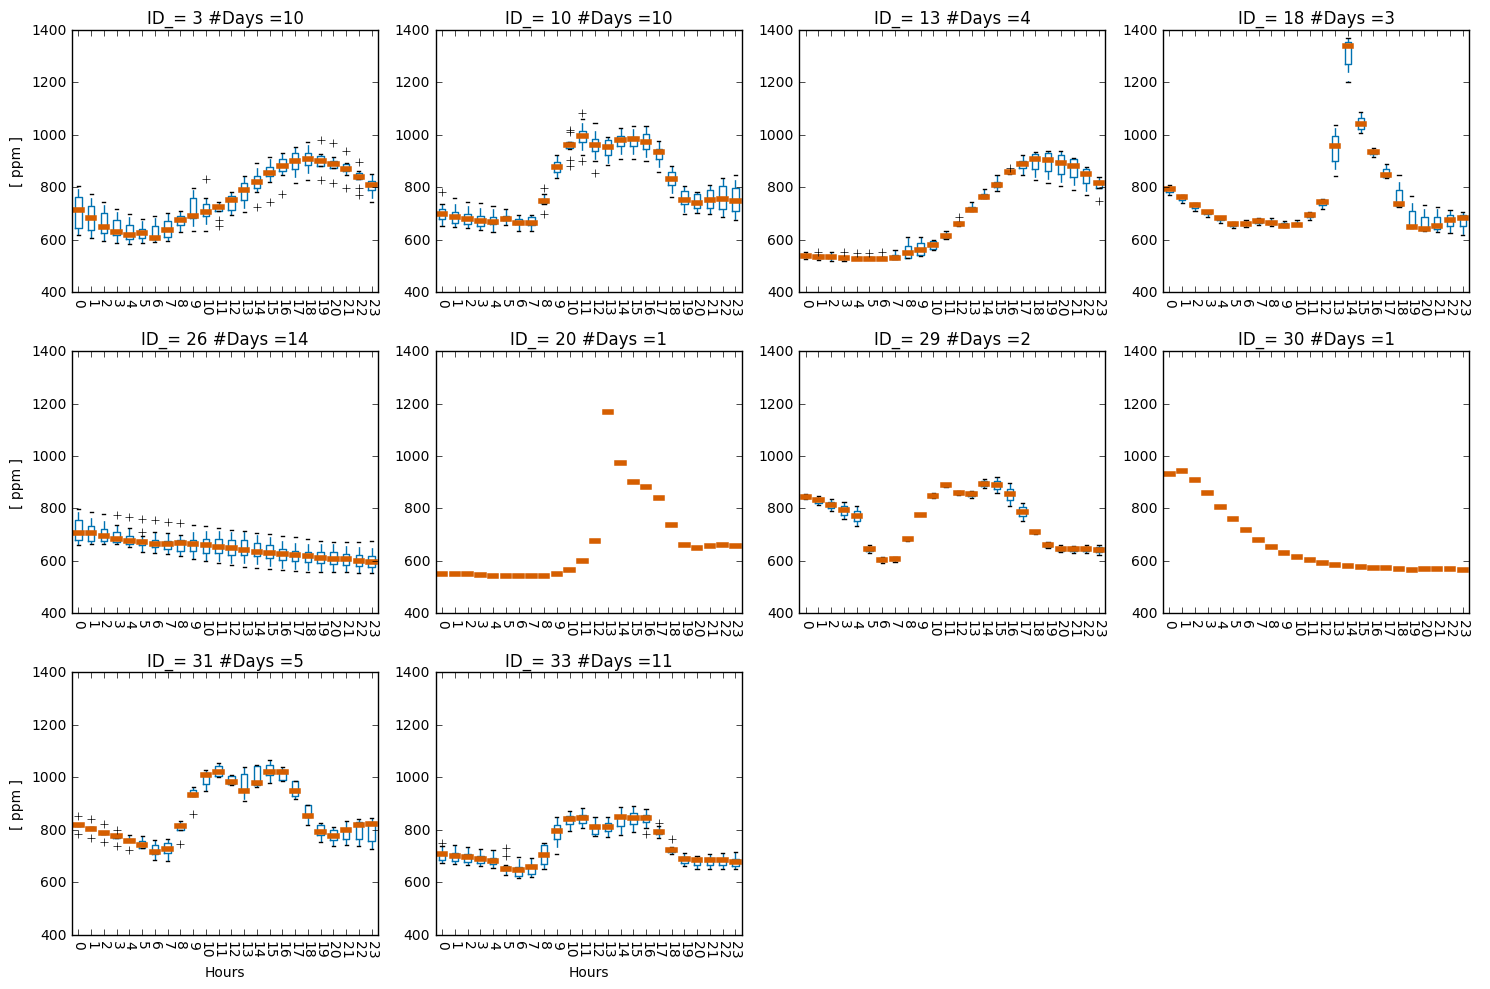
\includegraphics[scale=0.6]{Figures/discord_candidates_all.jpg}
  \caption{$CO_2$ discord clusters of the North-East ventilation system of the building. }
  \label{fig:discord_candidates_all}
\end{figure}

\begin{figure}[h!]
  \vspace{0.5em} %better style
  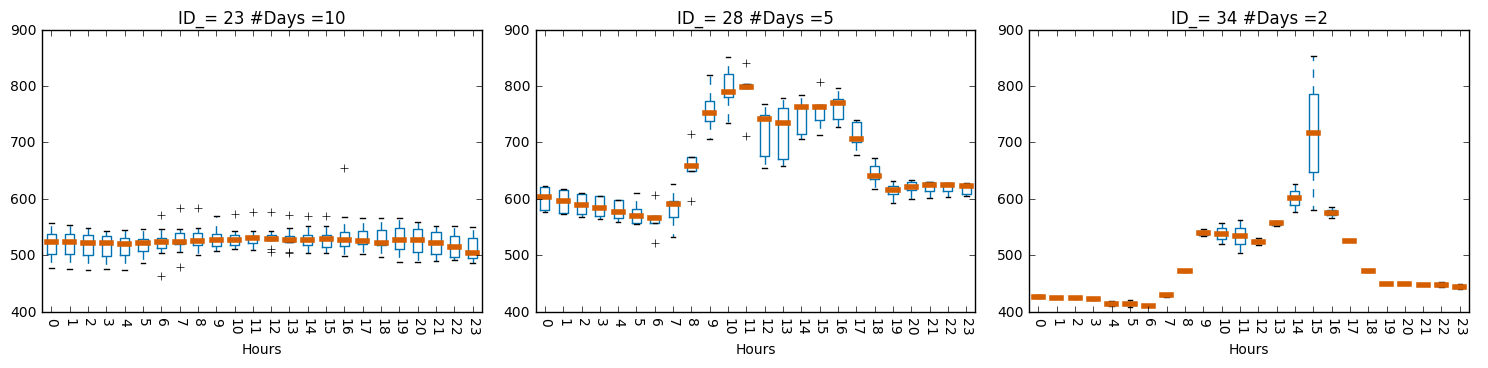
\includegraphics[scale=0.6]{Figures/discord_candidates_all_SW.jpg}
  \caption{$CO_2$ discord clusters of the South-West ventilation system of the building. }
  \label{fig:discord_candidates_all_SW}
\end{figure}

\end{landscape}
\restoregeometry


% Table generated by Excel2LaTeX from sheet 'SAX vs GaHMM'
\begin{table}[htbp]
  \centering
  \scriptsize
  \caption{Number of days where discords clusters were spotted by using \textit{GaHMM-profile model} and DayFilter approach. The corresponding coincidence of both approaches is done when both have the same date.}
  \begin{tabular}{|l|r|r|r|r|r|}
    \multicolumn{6}{c}{\textbf{CO2 level North East (V005\_vent01\_CO2)}} \bigstrut[b]\\
    \hline
         & \multicolumn{1}{l|}{\textbf{W = 4, |A|= 3}} & \multicolumn{1}{l|}{\textbf{W = 4, |A|= 4}} & \multicolumn{1}{l|}{\textbf{W = 4, |A|= 5}} & \multicolumn{1}{l|}{\textbf{W = 4, |A|= 6}} &  \bigstrut\\
    \hline
    \textbf{GaHMM} & 61   & 61   & 61   & 61   & days \bigstrut\\
    \hline
    \textbf{DayFilter} & 311  & 84   & 29   & 36   & days \bigstrut\\
    \hline
    \textbf{Coincidence} & 49   & 39   & 25   & 21   & days \bigstrut\\
    \hline
    \textbf{\% coincidence} & \cellcolor[rgb]{ .973,  .459,  .427} 15.2 & \cellcolor[rgb]{ .937,  .906,  .518} 36.8 & \cellcolor[rgb]{ .894,  .894,  .514} 38.5 & \cellcolor[rgb]{ .988,  .757,  .482} 27.6 & \% \bigstrut\\
    \hline
    \multicolumn{1}{r}{} & \multicolumn{1}{r}{} & \multicolumn{1}{r}{} & \multicolumn{1}{r}{} & \multicolumn{1}{r}{} & \multicolumn{1}{r}{} \bigstrut\\
    \hline
         & \multicolumn{1}{l|}{\textbf{W = 6, |A|= 3}} & \multicolumn{1}{l|}{\textbf{W = 6, |A|= 4}} & \multicolumn{1}{l|}{\textbf{W = 6, |A|= 5}} & \multicolumn{1}{l|}{\textbf{W = 6, |A|= 6}} &  \bigstrut\\
    \hline
    \textbf{GaHMM} & 61   & 61   & 61   & 61   & days \bigstrut\\
    \hline
    \textbf{DayFilter} & 49   & 33   & 19   & 16   & days \bigstrut\\
    \hline
    \textbf{Coincidence} & 29   & 25   & 17   & 15   & days \bigstrut\\
    \hline
    \textbf{\% coincidence} & \cellcolor[rgb]{ .965,  .914,  .518} 35.8 & \cellcolor[rgb]{ .953,  .91,  .518} 36.2 & \cellcolor[rgb]{ .988,  .741,  .482} 27.0 & \cellcolor[rgb]{ .984,  .675,  .467} 24.2 & \% \bigstrut\\
    \hline
    \multicolumn{1}{r}{} & \multicolumn{1}{r}{} & \multicolumn{1}{r}{} & \multicolumn{1}{r}{} & \multicolumn{1}{r}{} & \multicolumn{1}{r}{} \bigstrut[t]\\
    \multicolumn{6}{c}{\textbf{Temperature room 101 (V044\_room101\_temp)}} \bigstrut[b]\\
    \hline
         & \multicolumn{1}{l|}{\textbf{W = 4, |A|= 3}} & \multicolumn{1}{l|}{\textbf{W = 4, |A|= 4}} & \multicolumn{1}{l|}{\textbf{W = 4, |A|= 5}} & \multicolumn{1}{l|}{\textbf{W = 4, |A|= 6}} &  \bigstrut\\
    \hline
    \textbf{GaHMM} & 114  & 114  & 114  & 114  & days \bigstrut\\
    \hline
    \textbf{DayFilter} & 319  & 145  & 120  & 99   & days \bigstrut\\
    \hline
    \textbf{Coincidence} & 114  & 87   & 85   & 68   & days \bigstrut\\
    \hline
    \textbf{\% coincidence} & \cellcolor[rgb]{ .969,  .914,  .518} 35.7 & \cellcolor[rgb]{ .565,  .796,  .494} 50.6 & \cellcolor[rgb]{ .388,  .745,  .482} 57.0 & \cellcolor[rgb]{ .667,  .827,  .502} 46.9 & \% \bigstrut\\
    \hline
    \multicolumn{1}{r}{} & \multicolumn{1}{r}{} & \multicolumn{1}{r}{} & \multicolumn{1}{r}{} & \multicolumn{1}{r}{} & \multicolumn{1}{r}{} \bigstrut\\
    \hline
         & \multicolumn{1}{l|}{\textbf{W = 6, |A|= 3}} & \multicolumn{1}{l|}{\textbf{W = 6, |A|= 4}} & \multicolumn{1}{l|}{\textbf{W = 6, |A|= 5}} & \multicolumn{1}{l|}{\textbf{W = 6, |A|= 6}} &  \bigstrut\\
    \hline
    \textbf{GaHMM} & 114  & 114  & 114  & 114  & days \bigstrut\\
    \hline
    \textbf{DayFilter} & 209  & 138  & 109  & 95   & days \bigstrut\\
    \hline
    \textbf{Coincidence} & 102  & 85   & 74   & 70   & days \bigstrut\\
    \hline
    \textbf{\% coincidence} & \cellcolor[rgb]{ .686,  .831,  .502} 46.2 & \cellcolor[rgb]{ .557,  .796,  .494} 50.9 & \cellcolor[rgb]{ .588,  .804,  .494} 49.7 & \cellcolor[rgb]{ .573,  .8,  .494} 50.4 & \% \bigstrut\\
    \hline
    \multicolumn{1}{r}{} & \multicolumn{1}{r}{} & \multicolumn{1}{r}{} & \multicolumn{1}{r}{} & \multicolumn{1}{r}{} & \multicolumn{1}{r}{} \bigstrut[t]\\
    \multicolumn{6}{c}{\textbf{Humidity room 101 (V043\_room101\_hum)}} \bigstrut[b]\\
    \hline
         & \multicolumn{1}{l|}{\textbf{W = 4, |A|= 3}} & \multicolumn{1}{l|}{\textbf{W = 4, |A|= 4}} & \multicolumn{1}{l|}{\textbf{W = 4, |A|= 5}} & \multicolumn{1}{l|}{\textbf{W = 4, |A|= 6}} &  \bigstrut\\
    \hline
    \textbf{GaHMM} & 74   & 74   & 74   & 74   & days \bigstrut\\
    \hline
    \textbf{DayFilter} & 562  & 357  & 259  & 215  & days \bigstrut\\
    \hline
    \textbf{Coincidence} & 74   & 73   & 72   & 72   & days \bigstrut\\
    \hline
    \textbf{\% coincidence} & \cellcolor[rgb]{ .973,  .412,  .42} 13.2 & \cellcolor[rgb]{ .98,  .584,  .451} 20.4 & \cellcolor[rgb]{ .988,  .757,  .482} 27.6 & \cellcolor[rgb]{ .996,  .89,  .51} 33.2 & \% \bigstrut\\
    \hline
    \multicolumn{1}{r}{} & \multicolumn{1}{r}{} & \multicolumn{1}{r}{} & \multicolumn{1}{r}{} & \multicolumn{1}{r}{} & \multicolumn{1}{r}{} \bigstrut\\
    \hline
         & \multicolumn{1}{l|}{\textbf{W = 6, |A|= 3}} & \multicolumn{1}{l|}{\textbf{W = 6, |A|= 4}} & \multicolumn{1}{l|}{\textbf{W = 6, |A|= 5}} & \multicolumn{1}{l|}{\textbf{W = 6, |A|= 6}} &  \bigstrut\\
    \hline
    \textbf{GaHMM} & 74   & 74   & 74   & 74   & days \bigstrut\\
    \hline
    \textbf{DayFilter} & 523  & 328  & 238  & 204  & days \bigstrut\\
    \hline
    \textbf{Coincidence} & 73   & 73   & 72   & 72   & days \bigstrut\\
    \hline
    \textbf{\% coincidence} & \cellcolor[rgb]{ .973,  .427,  .42} 13.9 & \cellcolor[rgb]{ .976,  .529,  .439} 18.2 & \cellcolor[rgb]{ .984,  .647,  .463} 23.1 & \cellcolor[rgb]{ .988,  .714,  .475} 25.9 & \% \bigstrut\\
    \hline
    \end{tabular}%   
  \label{tab:SAXvsGaHMM_all}%
\end{table}%








\newgeometry{margin=1.5cm}
\begin{landscape}
\leavevmode
\newline

\subsection{Case Study}
\begin{figure}[h!]
  \vspace{0.5em} %better style
  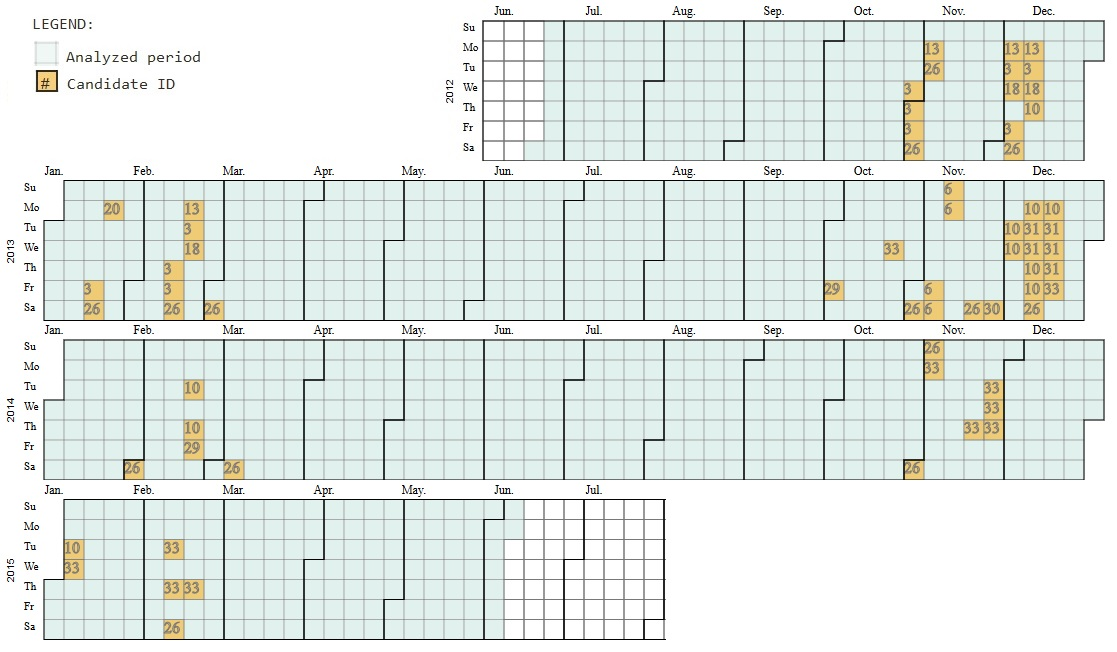
\includegraphics[scale=0.8]{Figures/Fault_id_candidate.jpg}
  \caption{Sequence of $CO_2$ discord clusters of the North-East ventilation system. Cluster 26 appears in mostly all the fault periods. }
  \label{fig:sequence_candidates}
\end{figure}

\begin{figure}[h!]
  \vspace{0.5em} %better style
  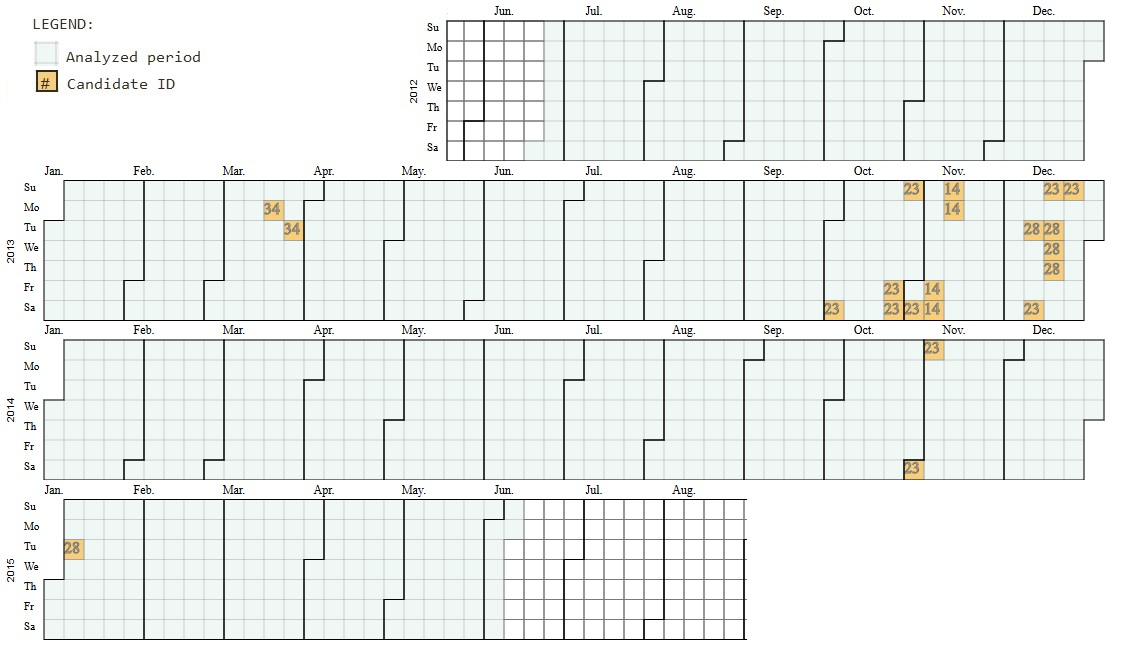
\includegraphics[scale=0.87]{Figures/Fault_id_candidate_SW.jpg}
  \caption{Sequence of $CO_2$ discord clusters of the South-West ventilation system. }
  \label{fig:sequence_candidates_SW}
\end{figure}

\end{landscape}
\restoregeometry

\pagebreak

\newgeometry{margin=1.5cm}
\begin{landscape}
\leavevmode
\newline

\subsection{Coincidence between FilterDay and GaHMM-profile model}
\label{viz:FilterDay_GaHMM}
\begin{figure}[h!]
  \vspace{0.5em} %better style
  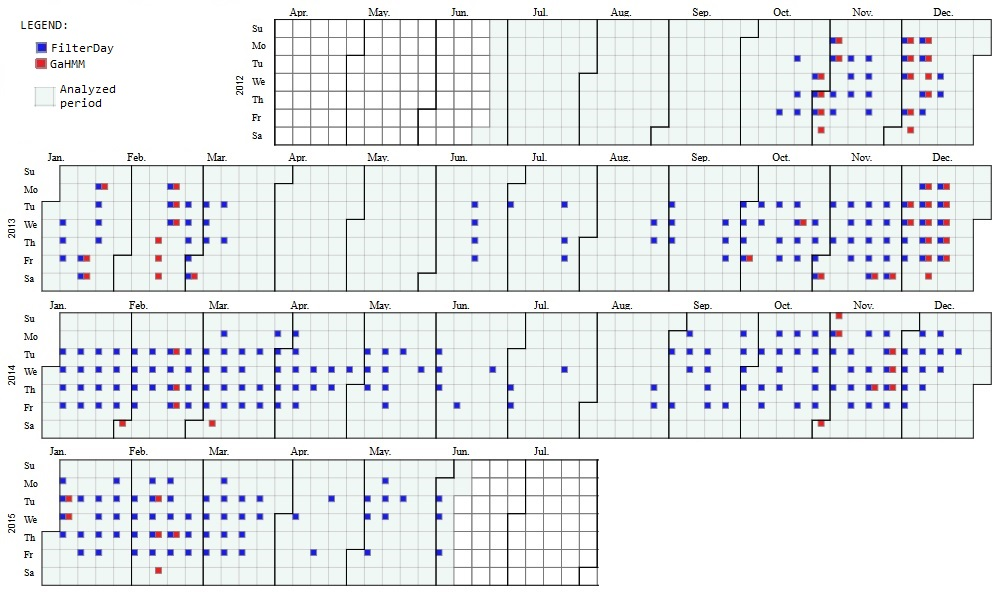
\includegraphics[scale=0.7]{Figures/GaHMMvsSAX_w4a3.jpg}
  \caption{Coincidence FilterDay vs. GaHMM-profile when $W=4, |A|=3$. A small square indicates a $CO_2$ daily profile spotted as discord cluster for the North-East ventilation system.}
  \label{fig:FilterDay_GaHMM_calendar1}
\end{figure}
\end{landscape}
\restoregeometry
    

\newgeometry{margin=1.5cm}
\begin{landscape}
\leavevmode
\newline

\begin{figure}[h!]
  \vspace{0.5em} %better style
  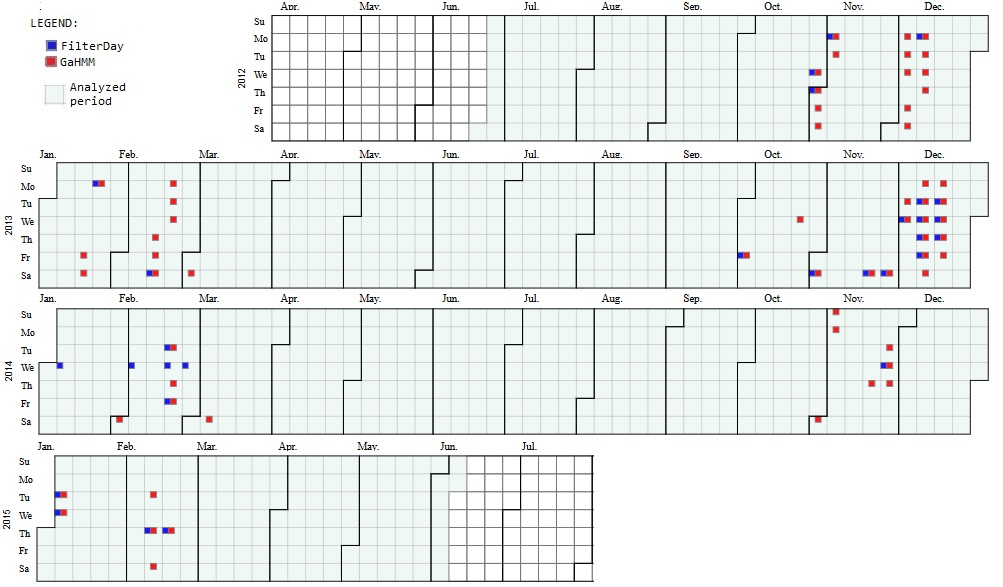
\includegraphics[scale=0.80]{Figures/GaHMMvsSAX_w4a5.jpg}
  \caption{Coincidence FilterDay vs. GaHMM-profile when $W=4, |A|=5$. A small square indicates a $CO_2$ daily profile spotted as discord cluster for the North-East ventilation system.}
  \label{fig:FilterDay_GaHMM_calendar2}
\end{figure}





\end{landscape}
\restoregeometry








% Table generated by Excel2LaTeX from sheet 'Dates Fault in NE vent system'
\begin{table}[htbp]
  \centering
  \scriptsize
  \caption{Dates when the $CO_2$ discord clusters of the North-East ventilation system were spotted by using the \textit{GaHMM-profile model} approach.}
    \begin{tabular}{|c|l|}
    \hline
    \rowcolor[rgb]{ .851,  .851,  .851} \textbf{ID cluster} & \multicolumn{1}{c|}{\textbf{Date (yyyy-mm-dd)}} \bigstrut\\
    \hline
    3    & 2012-10-31, 2012-11-01, 2012-11-02, 2012-12-04, 2012-12-07, 2012-12-11, 2013-01-18, \bigstrut[t]\\
         & 2013-02-14, 2013-02-15, 2013-02-19 \bigstrut[b]\\
    \hline
    \rowcolor[rgb]{ .949,  .949,  .949} 10   & 2012-12-13, 2013-12-03, 2013-12-04, 2013-12-09, 2013-12-12, 2013-12-13, \bigstrut[t]\\
    \rowcolor[rgb]{ .949,  .949,  .949}      & 2013-12-16, 2014-02-18, 2014-02-20, 2015-01-06 \bigstrut[b]\\
    \hline
    13   & 2012-11-05, 2012-12-03, 2012-12-10, 2013-02-18 \bigstrut\\
    \hline
    18   & 2012-12-05, 2012-12-12, 2013-02-20 \bigstrut\\
    \hline
    \rowcolor[rgb]{ .949,  .949,  .949} 26   & 2012-11-03, 2012-11-06, 2012-12-08, 2013-01-19, 2013-02-16, 2013-03-02, 2013-11-02,  \bigstrut[t]\\
    \rowcolor[rgb]{ .949,  .949,  .949}      & 2013-11-23, 2013-12-14, 2014-02-01, 2014-03-08, 2014-11-01, 2014-11-02, 2015-02-14 \bigstrut[b]\\
    \hline
    20   & 2013-01-21 \bigstrut\\
    \hline
    29   & 2013-10-04, 2014-02-21 \bigstrut\\
    \hline
    \rowcolor[rgb]{ .949,  .949,  .949} 30   & 2013-11-30 \bigstrut\\
    \hline
    31   & 2013-12-10, 2013-12-11, 2013-12-17, 2013-12-18, 2013-12-19 \bigstrut\\
    \hline
    33   & 2013-10-23, 2013-12-20, 2014-11-03, 2014-11-20, 2014-11-25, 2014-11-26, 2014-11-27, \bigstrut[t]\\
         &  2015-01-07, 2015-02-10, 2015-02-12, 2015-02-19 \bigstrut[b]\\
    \hline
    \end{tabular}%
  \label{tab:dates_NE_CO2_ventilation}%
\end{table}%


